% interacttfssample.tex
% v1.05 - August 2017

%\RequirePackage[2020/02/10]{latexrelease}
\let\negmedspace\undefined
\let\negthickspace\undefined

\documentclass[]{interact}
\usepackage{amsmath}
 \usepackage{amssymb}
 \usepackage{gensymb}
 \usepackage{tikz}
 \usepackage{enumitem}
 \usepackage{listings}
 \usepackage{color}                                            %%
 \usepackage{array}                                            %%
 \usepackage{longtable}                                        %%
 \usepackage{calc}                                             %%
 \usepackage{multirow}                                         %%
 \usepackage{hhline}                                           %%
 \usepackage{ifthen}                                           %%
%optionally (for landscape tables embedded in another document): %%
 \usepackage{lscape}     
\usepackage{multicol}
\usepackage{chngcntr}

\usepackage{epstopdf}% To incorporate .eps illustrations using PDFLaTeX, etc.
\usepackage[caption=false]{subfig}% Support for small, `sub' figures and tables
%\usepackage[nolists,tablesfirst]{endfloat}% To `separate' figures and tables from text if required

%\usepackage[doublespacing]{setspace}% To produce a `double spaced' document if required
%\setlength\parindent{24pt}% To increase paragraph indentation when line spacing is doubled
%\setlength\bibindent{2em}% To increase hanging indent in bibliography when line spacing is doubled

\usepackage[numbers,sort&compress]{natbib}% Citation support using natbib.sty


  \usepackage{tkz-euclide} % loads  TikZ and tkz-base
%\usetkzobj{all}
 \usetikzlibrary{calc,math}
% \usetikzlibrary{fadings}

\bibpunct[, ]{[}{]}{,}{n}{,}{,}% Citation support using natbib.sty
\renewcommand\bibfont{\fontsize{10}{12}\selectfont}% Bibliography support using natbib.sty

\theoremstyle{plain}% Theorem-like structures provided by amsthm.sty
\newtheorem{theorem}{Theorem}[section]
\newtheorem{lemma}[theorem]{Lemma}
\newtheorem{corollary}[theorem]{Corollary}
\newtheorem{proposition}[theorem]{Proposition}

\theoremstyle{definition}
\newtheorem{definition}[theorem]{Definition}
\newtheorem{example}[theorem]{Example}

\theoremstyle{remark}
\newtheorem{remark}{Remark}
\newtheorem{notation}{Notation}

\providecommand{\abs}[1]{\lvert#1\rvert}
\providecommand{\sbrak}[1]{\ensuremath{{}\left[#1\right]}}
\providecommand{\lsbrak}[1]{\ensuremath{{}\left[#1\right.}}
\providecommand{\rsbrak}[1]{\ensuremath{{}\left.#1\right]}}
\providecommand{\brak}[1]{\ensuremath{\left(#1\right)}}
\providecommand{\lbrak}[1]{\ensuremath{\left(#1\right.}}
\providecommand{\rbrak}[1]{\ensuremath{\left.#1\right)}}
\providecommand{\cbrak}[1]{\ensuremath{\left\{#1\right\}}}
\providecommand{\lcbrak}[1]{\ensuremath{\left\{#1\right.}}
\providecommand{\rcbrak}[1]{\ensuremath{\left.#1\right\}}}
\providecommand{\pr}[1]{\ensuremath{\Pr\left(#1\right)}}
\providecommand{\system}[1]{\overset{\mathcal{#1}}{ \longleftrightarrow}}
\providecommand{\norm}[1]{\left\lVert#1\right\rVert}
\newcommand{\myvec}[1]{\ensuremath{\begin{pmatrix}#1\end{pmatrix}}}
%\newcommand{\cmyvec}[1]{\ensuremath{\begin{pmatrix*}[c]#1\end{pmatrix*}}}
%\newcommand{\cmyvec}[1]{\ensuremath{\begin{pmatrix}[c]#1\end{pmatrix}}}
\newcommand{\mydet}[1]{\ensuremath{\begin{vmatrix}#1\end{vmatrix}}}
\DeclareMathOperator{\sign}{sign}
\newcommand*{\permcomb}[4][0mu]{{{}^{#3}\mkern#1#2_{#4}}}
\newcommand*{\perm}[1][-3mu]{\permcomb[#1]{P}}
\newcommand*{\comb}[1][-1mu]{\permcomb[#1]{C}}
\newcommand{\solution}{\noindent \textbf{Solution: }}
\let\vec\mathbf
\def\inputGnumericTable{}                                 %%

\begin{document}


\articletype{DRAFT}% Specify the article type or omit as appropriate

\title{A Matrix Approach to Conic Sections}

\author{
% \name{G.~V.~V.~Sharma\thanks{CONTACT G.~V.~V.~Sharma. Email: gadepall@ee.iith.ac.in}}
% \affil{EE Department, IIT Hyderabad, Kandi 502285, India}
}

\maketitle

\begin{abstract}
  Proofs of some theorems related to cyclic quadrilaterals are provided using coordinate geometry and trigonometry.  Through this approach, constructions and proofs using contradiction are avoided. 
\end{abstract}

\begin{keywords}
  cyclic quadrilateral, coordinate geometry, trigonometry
\end{keywords}


\section{Introduction}

% \begin{figure}[!ht]
%   \centering
% %  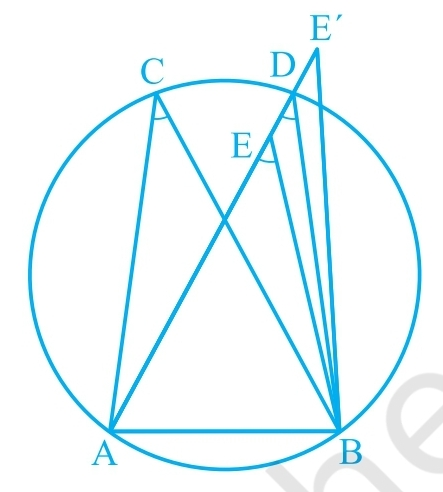
\includegraphics[width=\columnwidth]{figs/contra.jpg}
%   \resizebox{\columnwidth}{!}{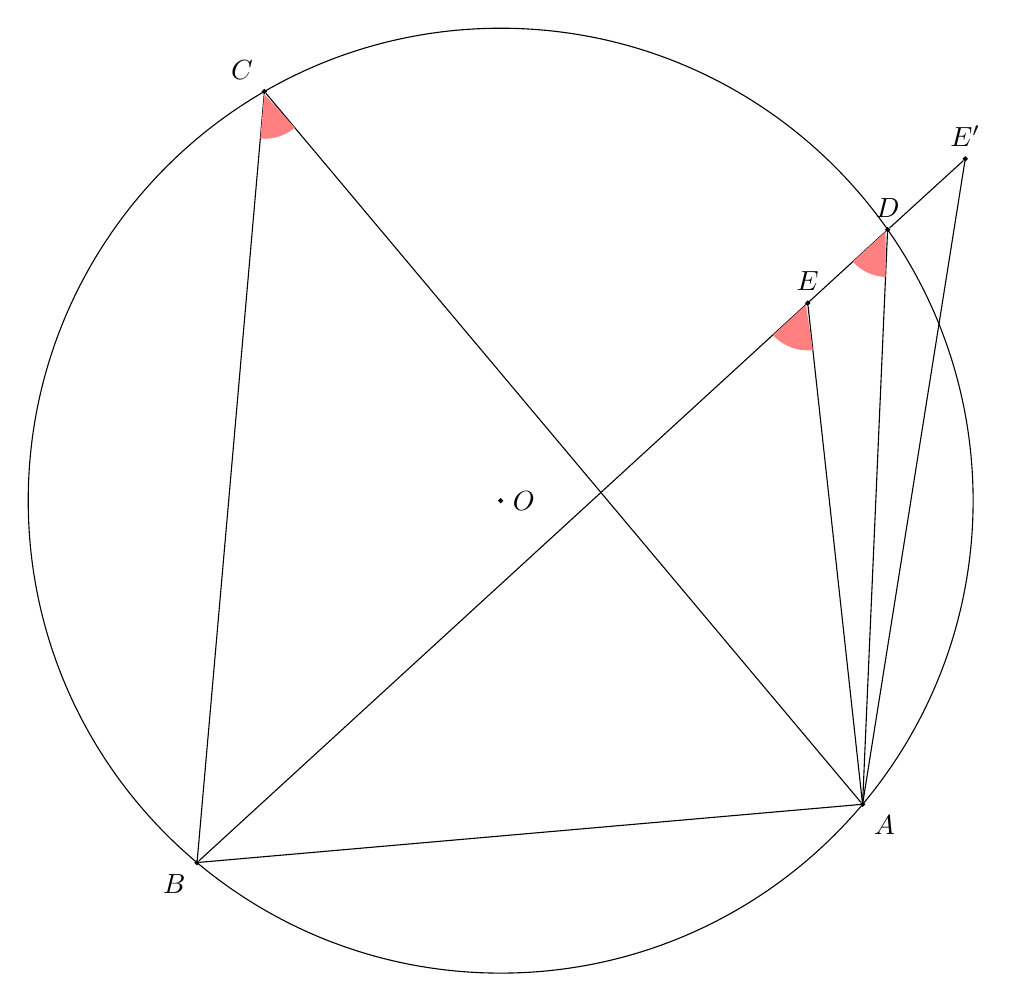
\begin{tikzpicture}
[scale=2,>=stealth,point/.style={draw,circle,fill = black,inner sep=0.5pt},]

%Polar Coordinates
\def\Ax{2.298}  %r=3 , theta1 = 320 degree
\def\Ay{-1.928}
\def\Bx{-1.928} %r=3 , theta2 = 230 degree
\def\By{-2.298}
\def\Cx{-1.5}  %r=3 , theta3 = 120 degree
\def\Cy{2.598}
\def\Dx{2.457}  %r=3 , theta4 =35 degree
\def\Dy{1.720}
\def\Ex{1.95}  
\def\Ey{1.254}
\def\Exn{2.95}
\def\Eyn{2.170}

%Labeling points
\node (A) at (\Ax,\Ay)[point,label=below right:$A$] {};
\node (B) at (\Bx,\By)[point,label=below left:$B$] {};
\node (C) at (\Cx,\Cy)[point,label=above left:$C$] {};
\node (D) at (\Dx,\Dy)[point,label=above :$D$] {};
\node (E) at (\Ex,\Ey)[point,label=above :$E$] {};
\node (En) at (\Exn,\Eyn)[point,label=above :$E'$] {};
\node (O) at (0,0)[point,label= right:$O$] {};

%Drawing lines
\draw (A) -- node[left] {} (B);
\draw (B) -- node[above] {} (C);
\draw (A) -- node[above] {} (D);
\draw (B) -- node[above] {} (D);
\draw (A) -- node[above] {} (C);
\draw (D) -- node[above] {} (En);
\draw (A) -- node[above] {} (En);
\draw (A) -- node[above] {} (E);

%Drawing angle
\tkzFillAngle[fill=red!50,size=.3](B,C,A)
\tkzFillAngle[fill=red!50,size=.3](B,E,A)
\tkzFillAngle[fill=red!50,size=.3](B,D,A)

%Drawing circle
\draw (O) circle (3);

\end{tikzpicture}
	

}
%   \caption{To show that $k = r$. }
%   \label{fig:8.5.13_C_circle_comp_contra}	
%   \end{figure}
  

\section{Preliminaries}
\begin{definition}
  The equation of a line passing through $\vec{x}_0$ in $\mathbb{R}^2$ is given by 
  \begin{align}
    \label{eq:line_norm_eq}
    \begin{aligned}[t]
  \vec{n}^{\top}\brak{\vec{x}-\vec{x}_0}&=0  &\brak{\text{normal form}}
  \\
  \text{or, } \vec{x}&=\vec{x}_0 + \lambda \vec{m}  & \brak{\text{parametric form}}
    \end{aligned}
\end{align}
%
where 
\begin{align}
  \vec{m} = \myvec{1 \\m}
\end{align}
is defined to be the {\em direction vector} of the line, $m$ being the slope and $\vec{n}$ defined by 
\begin{align}
  \vec{m}^{\top}\vec{n} = 0
  \label{eq:line_dir_norm}
\end{align}
%
is the {\em normal vector}.
\end{definition}
\begin{lemma}
  \label{conics/30/lemma}
  The distance of a point $\vec{P}$ from the line 
  \begin{align}
      \vec{n}^{\top}\vec{x}&=c  
\end{align}
is given by 
  \begin{align}
  d = \frac{\abs{\vec{n}^{\top}\vec{P}-c}}{\norm{\vec{n}}}   
  \end{align}
  \end{lemma}
\section{Vector Equation of a Conic Section}
\begin{definition}
  Let $\vec{P}$ be a point such that the ratio of its distance from a fixed point $\vec{F}$ and the distance ($d$) from a fixed line 
$L: \vec{n}^{\top}\vec{x}=c$ is constant, given by 
\label{conics/30/def}
\begin{align}
\frac{\norm{\vec{P}-\vec{F}}}{d} = e    
\end{align}
The locus of $\vec{P}$ such is known as a conic section. The line $L$ is known as the directrix and the point $\vec{F}$ is the focus. $e$ is defined to be 
the eccentricity of the conic.  
\begin{enumerate}
    \item For $e = 1$, the conic is a parabola
    \item For $e < 1$, the conic is an ellipse
    \item For $e > 1$, the conic is a hyperbola
\end{enumerate}
\end{definition}
\begin{theorem}
The equation of  a conic with directrix $\vec{n}^{\top}\vec{x} = c$, eccentricity $e$ and focus $\vec{F}$ is given by 
\begin{align}
    \label{eq:conic_quad_form}
    \vec{x}^{\top}\vec{V}\vec{x}+2\vec{u}^{\top}\vec{x}+f=0
    \end{align}
where     
\begin{align}
  \label{eq:conic_quad_form_v}
\vec{V} &=\norm{\vec{n}}^2\vec{I}-e^2\vec{n}\vec{n}^{\top}, 
\\
\label{eq:conic_quad_form_u}
\vec{u} &= ce^2\vec{n}-\norm{\vec{n}}^2\vec{F}, 
\\
\label{eq:conic_quad_form_f}
f &= \norm{\vec{n}}^2\norm{\vec{F}}^2-c^2e^2
%\\
    \end{align}
    
% \begin{align}
% \vec{x}^{\top}(t\vec{I}-\vec{n}\vec{n}^{\top})\vec{x}+2(c\vec{n}-t\vec{F})^{\top}\vec{x}+t\norm{\vec{F}}^2-c^2&=0
% \end{align}
%
%and 
% where 
% \begin{align}
%     %t=\frac{\norm{\vec{n}}^2}{e^2}
%     \norm{\vec{n}} = 1
% \end{align}
%\end{theorem}
\end{theorem}
\begin{proof}
  Using Definition \ref{conics/30/def} and Lemma \ref{conics/30/lemma},  for any point $\vec{x}$ on the conic,
\begin{align}
\norm{\vec{x}-\vec{F}}^2&=e^2 \frac{\brak{{\vec{n}^{\top}\vec{x} - c}}^2}{\norm{\vec{n}}^2}\label{conics/30/eq:1} \\
\implies \norm{\vec{n}}^2\brak{\vec{x}-\vec{F}}^{\top}\brak{\vec{x}-\vec{F}}&=e^2\brak{\vec{n}^{\top}\vec{x} - c}^2
\\
\implies \norm{\vec{n}}^2\brak{\vec{x}^{\top}\vec{x}-2\vec{F}^{\top}\vec{x}+\norm{\vec{F}}^2}&=e^2\brak{c^2+\brak{\vec{n}^{\top}\vec{x} }^2-2c\vec{n}^{\top}\vec{x}} \\
&=e^2\brak{c^2+\brak{\vec{x}^{\top}\vec{n}\vec{n}^{\top}\vec{x} }-2c\vec{n}^{\top}\vec{x}}
% t\vec{x}^{\top}\vec{x}-(\vec{n}^{\top}\vec{x} )^2-2t\vec{F}^{\top}\vec{x}+2c\vec{n}^{\top}\vec{x}=c^2-t\norm{\vec{F}}^2\\
% t\vec{x}^{\top}\vec{I}\vec{x}-\vec{n}^{\top}\vec{x} \vec{n}^{\top}\vec{x}+2(c\vec{n}-t\vec{F})^{\top}\vec{x}=c^2-t\norm{\vec{F}}^2\\
% \vec{x}^{\top}(t\vec{I}-\vec{n}\vec{n}^{\top})\vec{x}+2(c\vec{n}-t\vec{F})^{\top}\vec{x}+t\norm{\vec{F}}^2-c^2=0
\end{align}
%
which can be expressed as \eqref{eq:conic_quad_form} after simplification.

% See Appendix \ref{app:conicdef}
\end{proof}
%
\begin{lemma}
  \eqref{eq:conic_quad_form} represents a parabola for $\mydet{V} = 0 $, ellipse for $\mydet{V} > 0 $ and hyperbola for $\mydet{V} < 0 $.  In general
\eqref{eq:conic_quad_form}  represents a conic  if and only if
\begin{align}
\mydet{
\vec{V}&\vec{u}
\\
\vec{u}^{\top}&f
}
\ne  0
\label{eq:quad_forms_pair_det}
\end{align}
%
else, it represents a pair of straight lines.
\end{lemma}
%
\begin{example}
  \label{parab_ex1}
  The focus and  directrix of a parabola are given to be 
  \begin{align}
    \label{parab_ex1_F}
F &= \myvec{2\\3}
\\
\label{parab_ex1_nc}
\myvec{1 & -4}\vec{x} &= -3
  \end{align}
  From the given information,
  \begin{align}
    \vec{n} = \myvec{1\\-4}, c = -3, e = 1 
  \end{align}
Substituting in  \eqref{eq:conic_quad_form_v},  \eqref{eq:conic_quad_form_u} and  \eqref{eq:conic_quad_form_f},
\begin{align}
  \label{parab_ex1_V}
  \vec{V} &= (17)\myvec{1 & 0 \\ 0 & 1} - \myvec{1\\-4}\myvec{1 & -4} = \myvec{16 &  4 \\  4 & 1}
  \\
  \label{parab_ex1_u}
  \vec{u} &= (-3) \myvec{1\\-4}-(17)\myvec{2\\3} = \myvec{-37\\-39}
  \\
  \label{parab_ex1_f}
  f &= (17)(13)-(9) = 212
  \end{align}
which is exactly the same as \cite[Article 199, p. 176]{loney_coord}
\end{example}
%
\begin{example}
  \label{ellipse_ex1}
  The focus,  directrix and eccentricity of an ellipse  are given by 
  \begin{align}
    \label{ellipse_ex1_F}
F &= \myvec{-2\\3}
\\
\label{ellipse_ex1_nc}
\myvec{2 & 3}\vec{x} &= -4
\\
\label{ellipse_ex1_e}
e &= \frac{4}{5}
  \end{align}
  Substituting in  \eqref{eq:conic_quad_form_v},  \eqref{eq:conic_quad_form_u} and  \eqref{eq:conic_quad_form_f},
  \begin{align}
    \label{ellipse_ex1_V}
    \vec{V} &= (13)\myvec{1 & 0 \\ 0 & 1} -\brak{\frac{4}{5}}^2 \myvec{2\\3}\myvec{2 & 3} = \frac{1}{25}\myvec{261 & -96\\-96 & 181}
    \\
    \label{ellipse_ex1_u}
    \vec{u} &= (-4) \brak{\frac{4}{5}}^2\myvec{2\\3}-(13)\myvec{-2\\3} = \frac{1}{25}\myvec{ 522\\-1167}
    \\
    \label{ellipse_ex1_f}
    f &= (13)(13)-(16)\brak{\frac{4}{5}}^2 =\frac{3969}{25}
    \end{align}
  which matches \cite[Article 249, p. 227]{loney_coord}
  \end{example}
  

\section{Conic Parameters }
\subsection{Through  Eigenvalue Decomposition}
\begin{theorem}
  The conic in     \eqref{eq:conic_quad_form} can be expressed in standard form (centre/vertex at the origin, major axis - $x$ axis) as
  \begin{align}
    %\begin{aligned}
    \label{eq:conic_simp_temp_nonparab}
    \vec{y}^{\top}\vec{D}\vec{y} &=  \vec{u}^{\top}\vec{V}^{-1}\vec{u} -f  &  \abs{V} &\ne 0
    \\
    \vec{y}^{\top}\vec{D}\vec{y} &=  -2\eta\vec{e}_1^{\top}\vec{y}   & \abs{V} &= 0
    \label{eq:conic_simp_temp_parab}
    %\end{aligned}
    \end{align}

    where
    \begin{align}
      %\begin{split}
      \label{eq:conic_parmas_eig_def}
      \vec{P}^{\top}\vec{V}\vec{P} &= \vec{D}. \quad \text{(Eigenvalue Decomposition)}
      \\
      \vec{D} &= \myvec{\lambda_1 & 0\\ 0 & \lambda_2}, 
      \\
      \vec{P} &= \myvec{\vec{p}_1 & \vec{p}_2}, \quad \vec{P}^{\top}=\vec{P}^{-1},
      \label{eq:eigevecP}
      \\
      \label{eq:eta}
       \eta &=\vec{u}^{\top}\vec{p}_1
       \\
       \vec{e}_1 &=\myvec{1 \\ 0}
      \end{align}
      
\end{theorem}
\begin{proof}
  See Appendix \ref{app:parab}.
  \end{proof}
  
\begin{corollary}
  The centre/vertex of the conic is given by 
  \begin{align}
    %\begin{aligned}[t]
    \label{eq:conic_nonparab_c}
    \vec{c} &= - \vec{V}^{-1}\vec{u} & \abs{V} &\ne 0
    \\
    \myvec{ \vec{u}^{\top}+\eta\vec{p}_1^{\top} \\ \vec{V}}\vec{c} &= \myvec{-f \\ \eta\vec{p}_1-\vec{u}}  &\abs{V} &= 0
    %\end{cases}
    %\end{aligned}
    \label{eq:conic_parab_c}
    \end{align}
\end{corollary}
\begin{proof}
%The centre/vertex of the conic section in \eqref{eq:conic_quad_form} is given by $\vec{c}$ in \eqref{eq:conic_nonparab_c} or \eqref{eq:conic_parab_c}.  This is because 
From \eqref{eq:conic_affine},
\begin{align}
\label{eq:conic_affine_inv}
\vec{y} = \vec{P}^{\top}\brak{\vec{x}-\vec{c}}
\end{align}
For the standard conic, $\vec{y} = \vec{0} $ is the centre/vertex and in \eqref{eq:conic_affine_inv}, 
\begin{align}
\label{eq:conic_centre}
\vec{y} = \vec{0} \implies \vec{x}=\vec{c}
\end{align}
\end{proof}

% \begin{corollary}
%   For a circle, the radius is given by 
%    \begin{align} \sqrt{\norm{\vec{u}}^{2} -f} \label{eq:conic_simp_temp_circ_rad} \end{align} 
% \end{corollary}
% \begin{proof}
%   For a circle, 
%   \begin{align}
%     \vec{V}=\vec{D}= \vec{P} = \vec{I}
%     \end{align}
%     and the centre is obtained from \eqref{eq:conic_nonparab_c}, \eqref{eq:conic_centre}
%     as
%     \begin{align}
%     \label{eq:conic_circ_centre}
%     \vec{c} = -\vec{u}
%     \end{align}
%     \eqref{eq:conic_simp_temp_nonparab}
%     becomes
%     \begin{align}
%     \vec{y}^{\top}\vec{y} &=  \norm{\vec{y}}^2=\brak{\sqrt{\vec{u}^{\top}\vec{u} -f}}^2
%     \label{eq:conic_simp_temp_circ}
%     \end{align}
%     yileding \eqref{eq:conic_simp_temp_circ_rad}.
%     %
%     \end{proof}
In the following, various parameters are directly obtained from the standard forms  in  \eqref{eq:conic_simp_temp_nonparab} and \eqref{eq:conic_simp_temp_parab}
and the results in \cite{kemh103}
\begin{corollary}
  The focal length of the parabola in \eqref{eq:conic_simp_temp_parab} is given by 
  \begin{align}
    \mydet{\frac{2\eta}{\lambda_2}} 
    %= \mydet{\frac{2\vec{u}^T\vec{p}_1}{\lambda_2}}.
    \label{eq:conic_parab_foc_len} 
    \end{align}    
    where $\lambda_2$ is the nonzero eigenvalue of $\vec{V}$ and $\eta$ is defined in \eqref{eq:eta}.
    % \begin{align}
    %   \eta = \vec{u}^T\vec{p}_1
    %   \end{align}
     \end{corollary}
\begin{proof}
%   From \eqref{eq:conic_parab_foc_len_temp}, by comparing the coefficients of $y_2^2$ and $y_1$, the focal length of the parabola is obtained as 
% \begin{align}
% \mydet{\frac{2\vec{u}^T\vec{p}_1}{\lambda_2}}.
% \label{eq:conic_parab_foc_len} 
% \end{align}
From \eqref{eq:conic_parab_foc_len_temp}, by comparing the coefficients of $y_2^2$ and $y_1$, the focal length of the parabola is obtained as     \eqref{eq:conic_parab_foc_len} 
\end{proof}
\begin{corollary}
  For $\mydet{V} \ne 0$, the lengths of the semi-major and semi-minor axes of the conic in \eqref{eq:conic_quad_form} are given by 
  \begin{align} 
    \label{eq:ellipse_axes}
  %  \begin{aligned}[t]
    \sqrt{\frac{\vec{u}^{\top}\vec{V}^{-1}\vec{u} -f}{\lambda_1}}, 
    \sqrt{\frac{\vec{u}^{\top}\vec{V}^{-1}\vec{u} -f}{\lambda_2}}. \quad \brak{\text{ellipse}}
    \\
%
       \sqrt{\frac{\vec{u}^{\top}\vec{V}^{-1}\vec{u} -f}{\lambda_1}}, 
       \sqrt{\frac{f-\vec{u}^{\top}\vec{V}^{-1}\vec{u}}{\lambda_2}}, \quad \brak{\text{hyperbola }}
%
  %\end{aligned}
  \label{eq:hyper_axes}
\end{align} 

\end{corollary}
\begin{proof}
  For \begin{align} \abs{\vec{V}} > 0, \quad \text{or, } \lambda_1 > 0, \lambda_2 > 0 
  \end{align} and \eqref{eq:conic_simp_temp_nonparab} becomes \begin{align} \lambda_1y_1^2 +\lambda_2y_2^2 = 
  \vec{u}^{\top}\vec{V}^{-1}\vec{u} -f \end{align} yielding        \eqref{eq:ellipse_axes}.  Similarly, \eqref{eq:hyper_axes} can be obtained for 
  \begin{align} 
    \label{eq:conic_hyper_cond}
    \abs{\vec{V}} 
    < 0, \quad \text{or, } \lambda_1 > 0, \lambda_2 < 0 \end{align}
\end{proof}
\begin{corollary}
  The equation of the minor and major  axes are respectively given by 
  \begin{align}
\vec{p}_i^{\top}\brak{\vec{x}-\vec{c}} = 0, i = 1,2
  \end{align}
\end{corollary}
%Given \eqref{eq:conic_quad_form}, from \eqref{eq:conic_quad_form_vuf}, it can be seen that 
%
\subsection{Through Vector Equation}
%
\begin{theorem}
  \label{them:conic_quad_form_encF}
The eccentricity, directrices and foci of \eqref{eq:conic_quad_form} are given by 
\begin{align}
  \label{eq:conic_quad_form_e} 
  e&= \sqrt{1-\frac{\lambda_1}{\lambda_2}}
\\
\label{eq:conic_quad_form_nc} 
  \vec{n}&= \sqrt{\lambda_2}\vec{p}_1,  
  c = 
  \begin{cases}
    \frac{e\vec{u}^{\top}\vec{n} \pm \sqrt{e^2\brak{\vec{u}^{\top}\vec{n}}^2-\lambda_2\brak{e^2-1}\brak{\norm{\vec{u}}^2 - \lambda_2 f}}}{\lambda_2e\brak{e^2-1}} & e \ne 1
    \\
    \frac{\norm{\vec{u}}^2 - \lambda_2 f   }{2e^2\vec{u}^{\top}\vec{n}} & e = 1
  \end{cases}
  \\
  \label{eq:conic_quad_form_F} 
  \vec{F}  &= \frac{ce^2\vec{n}-\vec{u}}{\lambda_2}
\end{align}  
% \begin{align}
% \end{align}

\end{theorem}
\begin{proof}
  From \eqref{eq:conic_quad_form_v},
  \begin{align}
    \vec{V}^{\top} \vec{V}&=\brak{\norm{\vec{n}}^2\vec{I}-e^2\vec{n}\vec{n}^{\top}}^{\top}\brak{\norm{\vec{n}}^2\vec{I}-e^2\vec{n}\vec{n}^{\top}}
    \\
    \implies \vec{V}^{2} &= \norm{\vec{n}}^4\vec{I}+e^4\vec{n}\vec{n}^{\top}\vec{n}\vec{n}^{\top}-2e^2\norm{\vec{n}}^2\vec{n}\vec{n}^{\top}
    \\
    &= \norm{\vec{n}}^4\vec{I} + e^4\norm{\vec{n}}^2\vec{n}\vec{n}^{\top} - 2e^2\norm{\vec{n}}^2\vec{n}\vec{n}^{\top}
    \\
    &= \norm{\vec{n}}^4\vec{I} + e^2\brak{e^2 - 2}\norm{\vec{n}}^2\vec{n}\vec{n}^{\top}
    \\
    &= \norm{\vec{n}}^4\vec{I} + \brak{e^2 - 2}\norm{\vec{n}}^2\brak{\norm{\vec{n}}^2\vec{I}- \vec{V}}
    \end{align}
%    
which can be expressed as
\begin{align}
  \vec{V}^{2} + \brak{e^2 - 2}\norm{\vec{n}}^2\vec{V} - \brak{e^2 - 1}\norm{\vec{n}}^4\vec{I}=0
  \label{eq:conic_quad_form_e_cayley}
\end{align}
Using the Cayley-Hamilton theorem, \eqref{eq:conic_quad_form_e_cayley} results in the characteristic equation, 
\begin{align}
  \lambda^{2} - \brak{2-e^2}\norm{\vec{n}}^2\lambda + \brak{1-e^2 }\norm{\vec{n}}^4&=0
  \\
  \implies \brak{\frac{\lambda}{\norm{\vec{n}}^2}}^2 - \brak{2-e^2 }\brak{\frac{\lambda}{\norm{\vec{n}}^2}} + \brak{1-e^2 } &= 0
  \\
  \implies \frac{\lambda}{\norm{\vec{n}}^2} = 1-e^2, 1&
  \\
  \text{or, }\lambda_2 = \norm{\vec{n}}^2, \lambda_1 = \brak{1-e^2}\lambda_2 &
  \label{eq:conic_quad_form_lam_cayley}
\end{align}
From   \eqref{eq:conic_quad_form_lam_cayley}, the eccentricity of \eqref{eq:conic_quad_form} is given by 
\eqref{eq:conic_quad_form_e}.   
%
% By inspection, we find that 
% \begin{align}
%   \frac{\lambda}}{\norm{\vec{n}}^2} = 1
%   \label{eq:conic_quad_form_lam2_cayley}
% \end{align}
%satisfies \eqref{eq:conic_quad_form_lam_cayley}.
Multiplying both sides of    \eqref{eq:conic_quad_form_v} by $\vec{n}$,
\begin{align}
\vec{V} \vec{n}&=\norm{\vec{n}}^2\vec{n}-e^2\vec{n}\vec{n}^{\top}\vec{n} 
\\
&=\norm{\vec{n}}^2\brak{1-e^2}\vec{n} 
 \\
% &=\frac{\lambda_1}{\lambda_2}\norm{\vec{n}}^2\vec{n} 
% \end{align}
% upon substituting from \eqref{eq:conic_quad_form_e}  and simplifying.  From the above, it is obvious that $\vec{n}$ is an eigenvector
% of $\vec{V}$.  Choosing 
% \begin{align}
%   \lambda_2 = \norm{\vec{n}}^2,
%   \label{eq:eigevecn_lam2}
% \end{align}  
% we obtain 
% \begin{align}
  &=\lambda_1 \vec{n} 
  \label{eq:eigevecn}
\end{align}  
from \eqref{eq:conic_quad_form_lam_cayley}
Thus,  $\lambda_1$ is the corresponding eigenvalue for $\vec{n}$.  From       \eqref{eq:eigevecP},   \eqref{eq:conic_quad_form_lam_cayley} and \eqref{eq:eigevecn}, 
\begin{align}
   \vec{n}&= \norm{\vec{n}}\vec{p}_1  = \sqrt{\lambda_2}\vec{p}_1 
\end{align}  
From \eqref{eq:conic_quad_form_u} and \eqref{eq:conic_quad_form_lam_cayley},
\begin{align}
%   \label{eq:conic_quad_form_v}
% \vec{V} &=\norm{\vec{n}}^2\vec{I}-e^2\vec{n}\vec{n}^{\top}, 
% \\
%\label{eq:conic_quad_form_u}
\vec{F}  &= \frac{ce^2\vec{n}-\vec{u}}{\lambda_2}
 \\
 \implies \norm{\vec{F}}^2  &= \frac{\brak{ce^2\vec{n}-\vec{u}}^{\top}\brak{ce^2\vec{n}-\vec{u}}}{\lambda_2^2}
 \\
 \implies \lambda_2^2\norm{\vec{F}}^2  &= c^2e^4\lambda_2-2ce^2\vec{u}^{\top}\vec{n}+\norm{\vec{u}}^2
 \label{eq:conic_quad_form_u_temp}
% f &= \norm{\vec{n}}^2\norm{\vec{F}}^2-c^2e^2
% %\\
    \end{align}
    Also, \eqref{eq:conic_quad_form_f} can be expressed as
    \begin{align}
    \lambda_2\norm{\vec{F}}^2 &= f+c^2e^2
    \label{eq:conic_quad_form_f_temp}
\end{align}
From  \eqref{eq:conic_quad_form_u_temp} and     \eqref{eq:conic_quad_form_f_temp},
\begin{align}
c^2e^4\lambda_2-2ce^2\vec{u}^{\top}\vec{n}+\norm{\vec{u}}^2 = \lambda_2\brak{f+c^2e^2}
\\
\implies \lambda_2e^2\brak{e^2-1}c^2-2ce^2\vec{u}^{\top}\vec{n}+\norm{\vec{u}}^2 - \lambda_2 f = 0
\\
\text{or, } c = 
\begin{cases}
  \frac{e\vec{u}^{\top}\vec{n} \pm \sqrt{e^2\brak{\vec{u}^{\top}\vec{n}}^2-\lambda_2\brak{e^2-1}\brak{\norm{\vec{u}}^2 - \lambda_2 f}}}{\lambda_2e\brak{e^2-1}} & e \ne 1
  \\
  \frac{\norm{\vec{u}}^2 - \lambda_2 f   }{2e^2\vec{u}^{\top}\vec{n}} & e = 1
\end{cases}
\end{align}
% For a parabola, $e = 1$, hence, 
% \begin{align}
%   \vec{V} \vec{n} = \vec{0}
%   \end{align}
%   which can be used to obtain $\vec{n}$.

\end{proof}
\begin{example}
In Example \ref{parab_ex1}, starting with the equation of the conic
\begin{align}
  \label{parab_ex1_conic}
  \vec{x}^{\top}\myvec{16 &  4 \\  4 & 1}\vec{x} + 
   2 \myvec{-37\\-39}\vec{x}+ 212 = 0
  \end{align}
  the eigenvector decomposition of 
  \begin{align}
    \vec{V} = \myvec{16 &  4 \\  4 & 1}
    \end{align}
    is given by 
    \begin{align}
    \label{parab_ex1_D}
      \vec{D} &= \myvec{0 &  0 \\  0 & 17} \implies \lambda_1 = 0, \lambda_2 = 17,
      \\
      \label{parab_ex1_P}
      \vec{P} &= \frac{1}{\sqrt{17}}\myvec{-1 &  4 \\  4 & 1} \implies \vec{p}_1 = \frac{1}{\sqrt{17}}\myvec{-1  \\  4 }, \vec{p}_2 = \frac{1}{\sqrt{17}}\myvec{4  \\  1 }
      \end{align}
%      
From \eqref{eq:conic_quad_form_e} and     \eqref{parab_ex1_D}, the eccentricity
\begin{align}
e = 1.
    \end{align}
    From \eqref{eq:conic_quad_form_nc} \eqref{parab_ex1_u} and \eqref{parab_ex1_f}, substituting $e = 1$,  
      \begin{align}
        \vec{n}&= \sqrt{17}\frac{1}{\sqrt{17}}\myvec{-1 \\  4 } = \myvec{-1 \\  4 }
        \\
        c &= \frac{\brak{37^2+39^2}^2 - (17) (212)   }{2\myvec{-37&-39}\myvec{-1 \\  4 }} = 3
     \end{align}  
     which are the parameters of the directrix in \eqref{parab_ex1_nc}.  Substituting the above values in \eqref{eq:conic_quad_form_F},
     \begin{align}
      \vec{F}  &= \frac{3\myvec{-1 \\  4 }+\myvec{37\\39}}{17} = \myvec{2\\3}
     \end{align}  
     which matches \eqref{parab_ex1_F}.  Thus, Theorem \ref{them:conic_quad_form_encF} is verified for the parabola in \eqref{parab_ex1_conic}.
\end{example}

\begin{example}
  In Example \ref{ellipse_ex1}, starting with the equation of the conic
  \begin{align}
    \label{ellipse_ex1_conic}
    \vec{x}^{\top}\myvec{261 & -96\\-96 & 181}\vec{x} + 
     2 \myvec{ 522\\-1167}\vec{x}+ 3969 = 0
    \end{align}
    the eigenvector decomposition of 
    \begin{align}
      \vec{V} = \myvec{261 & -96\\-96 & 181}
      \end{align}
      is given by 
      \begin{align}
      \label{ellipse_ex1_D}
        \vec{D} &= \myvec{0 &  0 \\  0 & 17} \implies \lambda_1 = 0, \lambda_2 = 17,
        \\
        \label{ellipse_ex1_P}
        \vec{P} &= \frac{1}{\sqrt{17}}\myvec{-1 &  4 \\  4 & 1} \implies \vec{p}_1 = \frac{1}{\sqrt{17}}\myvec{-1  \\  4 }, \vec{p}_2 = \frac{1}{\sqrt{17}}\myvec{4  \\  1 }
        \end{align}
  %      
  From \eqref{eq:conic_quad_form_e} and     \eqref{ellipse_ex1_D}, the eccentricity
  \begin{align}
  e = 1.
      \end{align}
      From \eqref{eq:conic_quad_form_nc} \eqref{ellipse_ex1_u} and \eqref{ellipse_ex1_f}, substituting $e = 1$,  
        \begin{align}
          \vec{n}&= \sqrt{17}\frac{1}{\sqrt{17}}\myvec{-1 \\  4 } = \myvec{-1 \\  4 }
          \\
          c &= \frac{\brak{37^2+39^2}^2 - (17) (212)   }{2\myvec{-37&-39}\myvec{-1 \\  4 }} = 3
       \end{align}  
       which are the parameters of the directrix in \eqref{ellipse_ex1_nc}.
  \end{example}
  
\section{ Tangent and Normal}
\begin{theorem}
  The points of intersection of the line 
\begin{align}
L: \quad \vec{x} = \vec{q} + \mu \vec{m} \quad \mu \in \mathbb{R}
\label{eq:conic_tangent}
\end{align}
with the conic section in \eqref{eq:conic_quad_form} are given by
\begin{align}
\vec{x}_i = \vec{q} + \mu_i \vec{m}
\end{align}
%
where
\begin{multline}
\mu_i = \frac{1}
{
\vec{m}^T\vec{V}\vec{m}
}
\lbrak{-\vec{m}^T\brak{\vec{V}\vec{q}+\vec{u}}}
\\
\pm
{\small
\rbrak{\sqrt{
\sbrak{
\vec{m}^T\brak{\vec{V}\vec{q}+\vec{u}}
}^2
-
\brak
{
\vec{q}^T\vec{V}\vec{q} + 2\vec{u}^T\vec{q} +f
}
\brak{\vec{m}^T\vec{V}\vec{m}}
}
}
}
\label{eq:tangent_roots}
\end{multline}


\end{theorem}
\begin{proof}
  Substituting \eqref{eq:conic_tangent}
in \eqref{eq:conic_quad_form}, 
\begin{align}
\brak{\vec{q} + \mu \vec{m}}^T\vec{V}\brak{\vec{q} + \mu \vec{m}}  + 2 \vec{u}^T\brak{\vec{q} + \mu \vec{m}}+f &= 0
\\
\implies \mu^2\vec{m}^T\vec{V}\vec{m} + 2 \mu\vec{m}^T\brak{\vec{V}\vec{q}+\vec{u}} 
+ \vec{q}^T\vec{V}\vec{q} + 2\vec{u}^T\vec{q} +f &= 0
\label{eq:conic_intercept}
\end{align}
Solving the above quadratic in \eqref{eq:conic_intercept}
yields \eqref{eq:tangent_roots}.
\end{proof}
\begin{corollary}
  If $L$ in \eqref{eq:conic_tangent} touches \eqref{eq:conic_quad_form} at exactly one point $\vec{q}$, 
  \begin{align}
  \vec{m}^T\brak{\vec{V}\vec{q}+\vec{u}} = 0
  \label{eq:conic_tangent_mq}
  \end{align}
\end{corollary}
\begin{proof}
  In this case, \eqref{eq:conic_intercept} has exactly one root.  Hence, 
  in \eqref{eq:tangent_roots}
  \begin{align}
  \sbrak{
  \vec{m}^T\brak{\vec{V}\vec{q}+\vec{u}}
  }^2 -\brak{\vec{m}^T\vec{V}\vec{m}}
  \brak
  {
  \vec{q}^T\vec{V}\vec{q} + 2\vec{u}^T\vec{q} +f
  } = 0                                                                                             
  \label{eq:conic_tangent_disc}
  \end{align}                    
  $\because \vec{q}$ is the point of contact, $\vec{q}$ satisfies \eqref{eq:conic_quad_form}
  and 
  \begin{align}
  \vec{q}^T\vec{V}\vec{q} + 2\vec{u}^T\vec{q} +f = 0
  \label{eq:conic_tangent_qquad}
  \end{align}
  Substituting \eqref{eq:conic_tangent_qquad} in \eqref{eq:conic_tangent_disc} and simplifying, we obtain \eqref{eq:conic_tangent_mq}.
\end{proof}
\begin{theorem}[Tangent]
  Given the point of contact $\vec{q}$, the equation of a tangent to \eqref{eq:conic_quad_form} is 
  \begin{align}
  \brak{\vec{V}\vec{q}+\vec{u}}^T\vec{x}+\vec{u}^T\vec{q}+f = 0
  \label{eq:conic_tangent_final}
  \end{align}
\end{theorem}
\begin{proof}
  The normal vector is obtained from \eqref{eq:conic_tangent_mq} and \eqref{eq:line_dir_norm}
  as
  %
  \begin{align}
  \label{eq:conic_normal_vec}
  \vec{n} = \vec{V}\vec{q}+\vec{u}
  \end{align}  
  From \eqref{eq:conic_normal_vec} and \eqref{eq:line_norm_eq}, the equation of the tangent is\begin{align}
    \brak{\vec{V}\vec{q}+\vec{u}}^T\brak{\vec{x}-\vec{q}} &=0
    \\
    \implies \brak{\vec{V}\vec{q}+\vec{u}}^T\vec{x}-\vec{q}^T\vec{V}\vec{q}-\vec{u}^T\vec{q} &= 0
    \end{align}
    which, upon substituting from \eqref{eq:conic_tangent_qquad} and simplifying yields \eqref{eq:conic_tangent}.
\end{proof}
\begin{theorem}
  If $\vec{V}^{-1}$ exists, given the normal vector $\vec{n}$, the tangent points of contact to \eqref{eq:conic_quad_form} are given by
\begin{align}
  \begin{split}
\vec{q}_i &= \vec{V}^{-1}\brak{\kappa_i \vec{n}-\vec{u}}, i = 1,2
\\
\text{where }\kappa_i &= \pm \sqrt{
\frac{
\vec{u}^T\vec{V}^{-1}\vec{u}-f
}
{
\vec{n}^T\vec{V}^{-1}\vec{n}
}
}
  \end{split}
\label{eq:conic_tangent_qk}
\end{align}
\end{theorem}
\begin{proof}
  From \eqref{eq:conic_normal_vec},
\begin{align}
\label{eq:conic_normal_vec_q}
 \vec{q} = \vec{V}^{-1}\brak{\kappa \vec{n}-\vec{u}}, \quad \kappa \in \mathbb{R}
\end{align}
Substituting \eqref{eq:conic_normal_vec_q}
in \eqref{eq:conic_tangent_qquad},
\begin{align}
\brak{\kappa \vec{n}-\vec{u}}^T\vec{V}^{-1}\brak{\kappa \vec{n}-\vec{u}} 
%\\
+ 2\vec{u}^T\vec{V}^{-1}\brak{\kappa \vec{n}-\vec{u}} +f &= 0
\\
\implies 
\kappa^2 \vec{n}^T\vec{V}^{-1}\vec{n} - \vec{u}^T\vec{V}^{-1}\vec{u} + f &=0
 \\
 \text{or, } \kappa = \pm \sqrt{\frac{\vec{u}^T\vec{V}^{-1}\vec{u}-f}{\vec{n}^T\vec{V}^{-1}\vec{n}}} &\label{eq:conic_normal_k}
\end{align}
%
%yileding 
Substituting \eqref{eq:conic_normal_k} in \eqref{eq:conic_normal_vec_q}
yields \eqref{eq:conic_tangent_qk}.
%
\end{proof}


\begin{theorem}
  If $\vec{V}$ is not invertible,  given the normal vector $\vec{n}$, the point of contact to \eqref{eq:conic_quad_form} is given by the matrix equation
\begin{align}
\label{eq:conic_tangent_q_eigen}
\begin{pmatrix}
\vec{u+\kappa \vec{n}}^T \\ \vec{V}
\end{pmatrix}
\vec{q} &= 
\begin{pmatrix}
-f
\\
\kappa\vec{n}-\vec{u}
\end{pmatrix}
\\
\text{where }  \kappa = \frac{\vec{p}_1^T\vec{u}}{\vec{p}_1^T\vec{n}}, \quad \vec{V}\vec{p}_1 &= 0
\label{eq:conic_tangent_qk_eigen}
\end{align}

\end{theorem}
\begin{proof}
  If $\vec{V}$ is non-invertible, it has a zero eigenvalue.  If the corresponding eigenvector is $\vec{p}_1$, then,
\begin{align}
\vec{V}\vec{p}_1 = 0
\label{eq:conic_zero_eigen}
\end{align}
From \eqref{eq:conic_normal_vec},
\begin{align}
\label{eq:conic_zero_eigen_normal}
\kappa \vec{n} &= \vec{V} \vec{q}+\vec{u}, \quad \kappa \in \mathbb{R}
\\
\implies \kappa \vec{p}_1^T\vec{n} &= \vec{p}_1^T\vec{V} \vec{q}+\vec{p}_1^T\vec{u}
\\
\text{or, } \kappa \vec{p}_1^T\vec{n} &= \vec{p}_1^T\vec{u},  \quad \because \vec{p}_1^T \vec{V} = 0, 
%\\
\quad 
\brak{\text{ from } \eqref{eq:conic_zero_eigen}}
%\label{eq:conic_normal_vec_q}
\end{align}
yielding $\kappa$ in \eqref{eq:conic_tangent_qk_eigen}. From \eqref{eq:conic_zero_eigen_normal},
\begin{align}
\kappa \vec{q}^T\vec{n} &= \vec{q}^T\vec{V} \vec{q}+\vec{q}^T\vec{u}
\\
\implies \kappa \vec{q}^T\vec{n} &= -f-\vec{q}^T\vec{u} \quad \text{from } \eqref{eq:conic_tangent_qquad},
\\
\text{or, } \brak{\kappa \vec{n}+\vec{u}}\vec{q} &= -f
\label{eq:conic_zero_eigen_normal_fq}
\end{align}
\eqref{eq:conic_zero_eigen_normal} can be expressed as
\begin{align}
\label{eq:conic_zero_eigen_normal_vq}
\vec{V} \vec{q} = \kappa \vec{n} - \vec{u}.
\end{align}
\eqref{eq:conic_zero_eigen_normal_fq} and \eqref{eq:conic_zero_eigen_normal_vq} clubbed together result in \eqref{eq:conic_tangent_q_eigen}.
\end{proof}
All the results related to conics are summarized in 
Table \ref{table:conics}.  
\begin{table*}[!t]
\centering
%%%%%%%%%%%%%%%%%%%%%%%%%%%%%%%%%%%%%%%%%%%%%%%%%%%%%%%%%%%%%%%%%%%%%%
%%                                                                  %%
%%  This is the header of a LaTeX2e file exported from Gnumeric.    %%
%%                                                                  %%
%%  This file can be compiled as it stands or included in another   %%
%%  LaTeX document. The table is based on the longtable package so  %%
%%  the longtable options (headers, footers...) can be set in the   %%
%%  preamble section below (see PRAMBLE).                           %%
%%                                                                  %%
%%  To include the file in another, the following two lines must be %%
%%  in the including file:                                          %%
%%        \def\inputGnumericTable{}                                 %%
%%  at the beginning of the file and:                               %%
%%        \input{name-of-this-file.tex}                             %%
%%  where the table is to be placed. Note also that the including   %%
%%  file must use the following packages for the table to be        %%
%%  rendered correctly:                                             %%
%%    \usepackage[latin1]{inputenc}                                 %%
%%    \usepackage{color}                                            %%
%%    \usepackage{array}                                            %%
%%    \usepackage{longtable}                                        %%
%%    \usepackage{calc}                                             %%
%%    \usepackage{multirow}                                         %%
%%    \usepackage{hhline}                                           %%
%%    \usepackage{ifthen}                                           %%
%%  optionally (for landscape tables embedded in another document): %%
%%    \usepackage{lscape}                                           %%
%%                                                                  %%
%%%%%%%%%%%%%%%%%%%%%%%%%%%%%%%%%%%%%%%%%%%%%%%%%%%%%%%%%%%%%%%%%%%%%%



%%  This section checks if we are begin input into another file or  %%
%%  the file will be compiled alone. First use a macro taken from   %%
%%  the TeXbook ex 7.7 (suggestion of Han-Wen Nienhuys).            %%
\def\ifundefined#1{\expandafter\ifx\csname#1\endcsname\relax}


%%  Check for the \def token for inputed files. If it is not        %%
%%  defined, the file will be processed as a standalone and the     %%
%%  preamble will be used.                                          %%
\ifundefined{inputGnumericTable}

%%  We must be able to close or not the document at the end.        %%
	\def\gnumericTableEnd{\end{document}}


%%%%%%%%%%%%%%%%%%%%%%%%%%%%%%%%%%%%%%%%%%%%%%%%%%%%%%%%%%%%%%%%%%%%%%
%%                                                                  %%
%%  This is the PREAMBLE. Change these values to get the right      %%
%%  paper size and other niceties.                                  %%
%%                                                                  %%
%%%%%%%%%%%%%%%%%%%%%%%%%%%%%%%%%%%%%%%%%%%%%%%%%%%%%%%%%%%%%%%%%%%%%%

	\documentclass[12pt%
			  %,landscape%
                    ]{report}
       \usepackage[latin1]{inputenc}
       \usepackage{fullpage}
       \usepackage{color}
       \usepackage{array}
       \usepackage{longtable}
       \usepackage{calc}
       \usepackage{multirow}
       \usepackage{hhline}
       \usepackage{ifthen}

	\begin{document}


%%  End of the preamble for the standalone. The next section is for %%
%%  documents which are included into other LaTeX2e files.          %%
\else

%%  We are not a stand alone document. For a regular table, we will %%
%%  have no preamble and only define the closing to mean nothing.   %%
    \def\gnumericTableEnd{}

%%  If we want landscape mode in an embedded document, comment out  %%
%%  the line above and uncomment the two below. The table will      %%
%%  begin on a new page and run in landscape mode.                  %%
%       \def\gnumericTableEnd{\end{landscape}}
%       \begin{landscape}


%%  End of the else clause for this file being \input.              %%
\fi

%%%%%%%%%%%%%%%%%%%%%%%%%%%%%%%%%%%%%%%%%%%%%%%%%%%%%%%%%%%%%%%%%%%%%%
%%                                                                  %%
%%  The rest is the gnumeric table, except for the closing          %%
%%  statement. Changes below will alter the table's appearance.     %%
%%                                                                  %%
%%%%%%%%%%%%%%%%%%%%%%%%%%%%%%%%%%%%%%%%%%%%%%%%%%%%%%%%%%%%%%%%%%%%%%

\providecommand{\gnumericmathit}[1]{#1} 
%%  Uncomment the next line if you would like your numbers to be in %%
%%  italics if they are italizised in the gnumeric table.           %%
%\renewcommand{\gnumericmathit}[1]{\mathit{#1}}
\providecommand{\gnumericPB}[1]%
{\let\gnumericTemp=\\#1\let\\=\gnumericTemp\hspace{0pt}}
 \ifundefined{gnumericTableWidthDefined}
        \newlength{\gnumericTableWidth}
        \newlength{\gnumericTableWidthComplete}
        \newlength{\gnumericMultiRowLength}
        \global\def\gnumericTableWidthDefined{}
 \fi
%% The following setting protects this code from babel shorthands.  %%
 \ifthenelse{\isundefined{\languageshorthands}}{}{\languageshorthands{english}}
%%  The default table format retains the relative column widths of  %%
%%  gnumeric. They can easily be changed to c, r or l. In that case %%
%%  you may want to comment out the next line and uncomment the one %%
%%  thereafter                                                      %%
\providecommand\gnumbox{\makebox[0pt]}
%%\providecommand\gnumbox[1][]{\makebox}

%% to adjust positions in multirow situations                       %%
\setlength{\bigstrutjot}{\jot}
\setlength{\extrarowheight}{\doublerulesep}

%%  The \setlongtables command keeps column widths the same across  %%
%%  pages. Simply comment out next line for varying column widths.  %%
\setlongtables

\setlength\gnumericTableWidth{%
	59pt+%
	50pt+%
	70pt+%
	76pt+%
	67pt+%
0pt}
\def\gumericNumCols{5}
\setlength\gnumericTableWidthComplete{\gnumericTableWidth+%
         \tabcolsep*\gumericNumCols*2+\arrayrulewidth*\gumericNumCols}
\ifthenelse{\lengthtest{\gnumericTableWidthComplete > \linewidth}}%
         {\def\gnumericScale{\ratio{\linewidth-%
                        \tabcolsep*\gumericNumCols*2-%
                        \arrayrulewidth*\gumericNumCols}%
{\gnumericTableWidth}}}%
{\def\gnumericScale{1}}

%%%%%%%%%%%%%%%%%%%%%%%%%%%%%%%%%%%%%%%%%%%%%%%%%%%%%%%%%%%%%%%%%%%%%%
%%                                                                  %%
%% The following are the widths of the various columns. We are      %%
%% defining them here because then they are easier to change.       %%
%% Depending on the cell formats we may use them more than once.    %%
%%                                                                  %%
%%%%%%%%%%%%%%%%%%%%%%%%%%%%%%%%%%%%%%%%%%%%%%%%%%%%%%%%%%%%%%%%%%%%%%

\ifthenelse{\isundefined{\gnumericColA}}{\newlength{\gnumericColA}}{}\settowidth{\gnumericColA}{\begin{tabular}{@{}p{59pt*\gnumericScale}@{}}x\end{tabular}}
\ifthenelse{\isundefined{\gnumericColB}}{\newlength{\gnumericColB}}{}\settowidth{\gnumericColB}{\begin{tabular}{@{}p{50pt*\gnumericScale}@{}}x\end{tabular}}
\ifthenelse{\isundefined{\gnumericColC}}{\newlength{\gnumericColC}}{}\settowidth{\gnumericColC}{\begin{tabular}{@{}p{70pt*\gnumericScale}@{}}x\end{tabular}}
\ifthenelse{\isundefined{\gnumericColD}}{\newlength{\gnumericColD}}{}\settowidth{\gnumericColD}{\begin{tabular}{@{}p{76pt*\gnumericScale}@{}}x\end{tabular}}
\ifthenelse{\isundefined{\gnumericColE}}{\newlength{\gnumericColE}}{}\settowidth{\gnumericColE}{\begin{tabular}{@{}p{67pt*\gnumericScale}@{}}x\end{tabular}}

{\footnotesize
\begin{tabular}[c]{%
	b{\gnumericColA}%
	b{\gnumericColB}%
	b{\gnumericColC}%
	b{\gnumericColD}%
	b{\gnumericColE}%
	}

%%%%%%%%%%%%%%%%%%%%%%%%%%%%%%%%%%%%%%%%%%%%%%%%%%%%%%%%%%%%%%%%%%%%%%
%%  The longtable options. (Caption, headers... see Goosens, p.124) %%
%	\caption{The Table Caption.}             \\	%
% \hline	% Across the top of the table.
%%  The rest of these options are table rows which are placed on    %%
%%  the first, last or every page. Use \multicolumn if you want.    %%

%%  Header for the first page.                                      %%
%	\multicolumn{5}{c}{The First Header} \\ \hline 
%	\multicolumn{1}{c}{colTag}	%Column 1
%	&\multicolumn{1}{c}{colTag}	%Column 2
%	&\multicolumn{1}{c}{colTag}	%Column 3
%	&\multicolumn{1}{c}{colTag}	%Column 4
%	&\multicolumn{1}{c}{colTag}	\\ \hline %Last column
%	\endfirsthead

%%  The running header definition.                                  %%
%	\hline
%	\multicolumn{5}{l}{\ldots\small\slshape continued} \\ \hline
%	\multicolumn{1}{c}{colTag}	%Column 1
%	&\multicolumn{1}{c}{colTag}	%Column 2
%	&\multicolumn{1}{c}{colTag}	%Column 3
%	&\multicolumn{1}{c}{colTag}	%Column 4
%	&\multicolumn{1}{c}{colTag}	\\ \hline %Last column
%	\endhead

%%  The running footer definition.                                  %%
%	\hline
%	\multicolumn{5}{r}{\small\slshape continued\ldots} \\
%	\endfoot

%%  The ending footer definition.                                   %%
%	\multicolumn{5}{c}{That's all folks} \\ \hline 
%	\endlastfoot
%%%%%%%%%%%%%%%%%%%%%%%%%%%%%%%%%%%%%%%%%%%%%%%%%%%%%%%%%%%%%%%%%%%%%%

\hhline{|-|-|-|-|-}
	 \multicolumn{1}{|p{\gnumericColA}|}%
	{\gnumericPB{\centering}\textbf{Conic}}
	&\multicolumn{1}{p{\gnumericColB}|}%
	{\gnumericPB{\centering}\textbf{Property}}
	&\multicolumn{1}{p{\gnumericColC}|}%
	{\gnumericPB{\centering}\textbf{Standard Form}}
	&\multicolumn{1}{p{\gnumericColD}|}%
	{\gnumericPB{\centering}\textbf{Standard Parameters}}
	&\multicolumn{1}{p{\gnumericColE}|}%
	{\gnumericPB{\centering}\textbf{Point(s) of Contact}}
\\
\hhline{|-----|}
	 \multicolumn{1}{|p{\gnumericColA}|}%
	{\gnumericPB{\centering}\textbf{Circle}}
	&\multicolumn{1}{p{\gnumericColB}|}%
	{\gnumericPB{\centering}$\vec{V} = \vec{I}$}
	&\multicolumn{1}{p{\gnumericColC}|}%
	{\setlength{\gnumericMultiRowLength}{0pt}%
	 \addtolength{\gnumericMultiRowLength}{\gnumericColC}%
	 \multirow{3}[1]{\gnumericMultiRowLength}{\parbox{\gnumericMultiRowLength}{%
	\scriptsize \gnumericPB{\centering}$\begin{array}{c}\frac{\vec{y}^T\vec{D}\vec{y}}{\vec{u}^T\vec{V}^{-1}\vec{u}-f} = 1
\\
\vec{D} = \myvec{\lambda_1 & 0 \\ 0 & \lambda_2}
\\
\vec{V} = \vec{P}\vec{D}\vec{P}^T
\\
\vec{P} = \myvec{\vec{p}_1 & \vec{p}_2}
\end{array}$}}}
	&\multicolumn{1}{p{\gnumericColD}|}%
	{\scriptsize \gnumericPB{\centering}$\begin{array}{c}\vec{c} = -\vec{u}, \\ r = \sqrt{\vec{u}^T\vec{u}-f}\end{array}$}
	&\multicolumn{1}{p{\gnumericColE}|}%
	{\setlength{\gnumericMultiRowLength}{0pt}%
	 \addtolength{\gnumericMultiRowLength}{\gnumericColE}%
	 \multirow{3}[1]{\gnumericMultiRowLength}{\parbox{\gnumericMultiRowLength}{%
\tiny	 \gnumericPB{\centering}\begin{multline*} \vec{q} = \vec{V}^{-1}\brak{\kappa \vec{n}-\vec{u}}
\\
\kappa = \pm \sqrt{\frac{\vec{u}^T\vec{V}^{-1}\vec{u}-f}{\vec{n}^T\vec{V}^{-1}\vec{n}}}
\end{multline*}}}}
\\
\hhline{|--|~|-|~}
	 \multicolumn{1}{|p{\gnumericColA}|}%
	{\gnumericPB{\centering}\textbf{Ellipse}}
	&\multicolumn{1}{p{\gnumericColB}|}%
	{\gnumericPB{\centering}$\begin{array}{c}\abs{\vec{V}} > 0 \\ \lambda_1 > 0, \lambda_2 < 0 \end{array}$}
	&\multicolumn{1}{p{\gnumericColC}|}%
	{}
	&\multicolumn{1}{p{\gnumericColD}|}%
	{\tiny \gnumericPB{\centering}$\begin{array}{c}\vec{c} = -\vec{V}^{-1}\vec{u},\\ 
axes = 
\begin{cases}\sqrt{\frac{\vec{u}^T\vec{V}^{-1}\vec{u}-f}{\lambda_1}} \\ \sqrt{\frac{\vec{u}^T\vec{V}^{-1}\vec{u}-f}{\lambda_2}} \end{cases}
\end{array}$}
	&\multicolumn{1}{p{\gnumericColE}|}%
	{}
\\
\hhline{|--|~|-|~}
	 \multicolumn{1}{|p{\gnumericColA}|}%
	{\gnumericPB{\centering}\textbf{Hyperbola}}
	&\multicolumn{1}{p{\gnumericColB}|}%
	{\gnumericPB{\centering}$\begin{array}{c}\abs{\vec{V}} < 0\\ \lambda_1 > 0, \lambda_2 < 0\end{array}$}
	&\multicolumn{1}{p{\gnumericColC}|}%
	{}
	&\multicolumn{1}{p{\gnumericColD}|}%
	{\tiny \gnumericPB{\centering}
$\begin{array}{c}\vec{c} = -\vec{V}^{-1}\vec{u}, \\ 
axes = 
\begin{cases}
\sqrt{\frac{\vec{u}^T\vec{V}^{-1}\vec{u}-f}{\lambda_1}}\\ \sqrt{\frac{f-\vec{u}^T\vec{V}^{-1}\vec{u}}{\lambda_2}}
\end{cases}
\end{array}$}
	&\multicolumn{1}{p{\gnumericColE}|}%
	{}
\\
\hhline{|-----|}
	 \multicolumn{1}{|p{\gnumericColA}|}%
	{\gnumericPB{\centering}\textbf{Parabola}}
	&\multicolumn{1}{p{\gnumericColB}|}%
	{\gnumericPB{\centering}$\begin{array}{c}\abs{\vec{V}} = 0 \\ \lambda_1 = 0 \end{array}$}
	&\multicolumn{1}{p{\gnumericColC}|}%
	{\tiny  $\vec{y}^T\vec{D}\vec{y} =  -2\eta\myvec{1 & 0}\vec{y}$}
	&\multicolumn{1}{p{\gnumericColD}|}%
	{\tiny \gnumericPB{\centering}{ \begin{multline*} 
\text{focal length} = \mydet{\frac{2\eta}{\lambda_2}}
\\ 
\myvec{ \vec{u}^T+\eta\vec{p}_1^T \\ \vec{V}}\vec{c} 
\\
= \myvec{-f \\ \eta\vec{p}_1-\vec{u}}
\\
\eta = \vec{p}_1^T\vec{u}
\end{multline*}}}
	&\multicolumn{1}{p{\gnumericColE}|}%
	{\tiny \gnumericPB{\centering}{ \begin{multline*}
\myvec{ \vec{u+\kappa \vec{n}}^T \\ \vec{V}}\vec{q} 
\\
= \myvec{-f
\\
\kappa\vec{n}-\vec{u}}
\\
\kappa = \frac{\vec{p_1}^T\vec{u}}{\vec{p_1}^T\vec{n}}
\end{multline*}}}
\\
\hhline{|-|-|-|-|-|}
\end{tabular}
}
\ifthenelse{\isundefined{\languageshorthands}}{}{\languageshorthands{\languagename}}
\gnumericTableEnd

%%%%%%%%%%%%%%%%%%%%%%%%%%%%%%%%%%%%%%%%%%%%%%%%%%%%%%%%%%%%%%%%%%%%%%%
%%                                                                  %%
%%  This is the header of a LaTeX2e file exported from Gnumeric.    %%
%%                                                                  %%
%%  This file can be compiled as it stands or included in another   %%
%%  LaTeX document. The table is based on the longtable package so  %%
%%  the longtable options (headers, footers...) can be set in the   %%
%%  preamble section below (see PRAMBLE).                           %%
%%                                                                  %%
%%  To include the file in another, the following two lines must be %%
%%  in the including file:                                          %%
%%        \def\inputGnumericTable{}                                 %%
%%  at the beginning of the file and:                               %%
%%        \input{name-of-this-file.tex}                             %%
%%  where the table is to be placed. Note also that the including   %%
%%  file must use the following packages for the table to be        %%
%%  rendered correctly:                                             %%
%%    \usepackage[latin1]{inputenc}                                 %%
%%    \usepackage{color}                                            %%
%%    \usepackage{array}                                            %%
%%    \usepackage{longtable}                                        %%
%%    \usepackage{calc}                                             %%
%%    \usepackage{multirow}                                         %%
%%    \usepackage{hhline}                                           %%
%%    \usepackage{ifthen}                                           %%
%%  optionally (for landscape tables embedded in another document): %%
%%    \usepackage{lscape}                                           %%
%%                                                                  %%
%%%%%%%%%%%%%%%%%%%%%%%%%%%%%%%%%%%%%%%%%%%%%%%%%%%%%%%%%%%%%%%%%%%%%%



%%  This section checks if we are begin input into another file or  %%
%%  the file will be compiled alone. First use a macro taken from   %%
%%  the TeXbook ex 7.7 (suggestion of Han-Wen Nienhuys).            %%
\def\ifundefined#1{\expandafter\ifx\csname#1\endcsname\relax}


%%  Check for the \def token for inputed files. If it is not        %%
%%  defined, the file will be processed as a standalone and the     %%
%%  preamble will be used.                                          %%
\ifundefined{inputGnumericTable}

%%  We must be able to close or not the document at the end.        %%
	\def\gnumericTableEnd{\end{document}}


%%%%%%%%%%%%%%%%%%%%%%%%%%%%%%%%%%%%%%%%%%%%%%%%%%%%%%%%%%%%%%%%%%%%%%
%%                                                                  %%
%%  This is the PREAMBLE. Change these values to get the right      %%
%%  paper size and other niceties.                                  %%
%%                                                                  %%
%%%%%%%%%%%%%%%%%%%%%%%%%%%%%%%%%%%%%%%%%%%%%%%%%%%%%%%%%%%%%%%%%%%%%%

	\documentclass[12pt%
			  %,landscape%
                    ]{report}
       \usepackage[latin1]{inputenc}
       \usepackage{fullpage}
       \usepackage{color}
       \usepackage{array}
       \usepackage{longtable}
       \usepackage{calc}
       \usepackage{multirow}
       \usepackage{hhline}
       \usepackage{ifthen}

	\begin{document}


%%  End of the preamble for the standalone. The next section is for %%
%%  documents which are included into other LaTeX2e files.          %%
\else

%%  We are not a stand alone document. For a regular table, we will %%
%%  have no preamble and only define the closing to mean nothing.   %%
    \def\gnumericTableEnd{}

%%  If we want landscape mode in an embedded document, comment out  %%
%%  the line above and uncomment the two below. The table will      %%
%%  begin on a new page and run in landscape mode.                  %%
%       \def\gnumericTableEnd{\end{landscape}}
%       \begin{landscape}


%%  End of the else clause for this file being \input.              %%
\fi

%%%%%%%%%%%%%%%%%%%%%%%%%%%%%%%%%%%%%%%%%%%%%%%%%%%%%%%%%%%%%%%%%%%%%%
%%                                                                  %%
%%  The rest is the gnumeric table, except for the closing          %%
%%  statement. Changes below will alter the table's appearance.     %%
%%                                                                  %%
%%%%%%%%%%%%%%%%%%%%%%%%%%%%%%%%%%%%%%%%%%%%%%%%%%%%%%%%%%%%%%%%%%%%%%

\providecommand{\gnumericmathit}[1]{#1} 
%%  Uncomment the next line if you would like your numbers to be in %%
%%  italics if they are italizised in the gnumeric table.           %%
%\renewcommand{\gnumericmathit}[1]{\mathit{#1}}
\providecommand{\gnumericPB}[1]%
{\let\gnumericTemp=\\#1\let\\=\gnumericTemp\hspace{0pt}}
 \ifundefined{gnumericTableWidthDefined}
        \newlength{\gnumericTableWidth}
        \newlength{\gnumericTableWidthComplete}
        \newlength{\gnumericMultiRowLength}
        \global\def\gnumericTableWidthDefined{}
 \fi
%% The following setting protects this code from babel shorthands.  %%
 \ifthenelse{\isundefined{\languageshorthands}}{}{\languageshorthands{english}}
%%  The default table format retains the relative column widths of  %%
%%  gnumeric. They can easily be changed to c, r or l. In that case %%
%%  you may want to comment out the next line and uncomment the one %%
%%  thereafter                                                      %%
\providecommand\gnumbox{\makebox[0pt]}
%%\providecommand\gnumbox[1][]{\makebox}

%% to adjust positions in multirow situations                       %%
\setlength{\bigstrutjot}{\jot}
\setlength{\extrarowheight}{\doublerulesep}

%%  The \setlongtables command keeps column widths the same across  %%
%%  pages. Simply comment out next line for varying column widths.  %%
\setlongtables

\setlength\gnumericTableWidth{%
	59pt+%
	50pt+%
	70pt+%
	76pt+%
	67pt+%
0pt}
\def\gumericNumCols{5}
\setlength\gnumericTableWidthComplete{\gnumericTableWidth+%
         \tabcolsep*\gumericNumCols*2+\arrayrulewidth*\gumericNumCols}
\ifthenelse{\lengthtest{\gnumericTableWidthComplete > \linewidth}}%
         {\def\gnumericScale{\ratio{\linewidth-%
                        \tabcolsep*\gumericNumCols*2-%
                        \arrayrulewidth*\gumericNumCols}%
{\gnumericTableWidth}}}%
{\def\gnumericScale{1}}

%%%%%%%%%%%%%%%%%%%%%%%%%%%%%%%%%%%%%%%%%%%%%%%%%%%%%%%%%%%%%%%%%%%%%%
%%                                                                  %%
%% The following are the widths of the various columns. We are      %%
%% defining them here because then they are easier to change.       %%
%% Depending on the cell formats we may use them more than once.    %%
%%                                                                  %%
%%%%%%%%%%%%%%%%%%%%%%%%%%%%%%%%%%%%%%%%%%%%%%%%%%%%%%%%%%%%%%%%%%%%%%

\ifthenelse{\isundefined{\gnumericColA}}{\newlength{\gnumericColA}}{}\settowidth{\gnumericColA}{\begin{tabular}{@{}p{59pt*\gnumericScale}@{}}x\end{tabular}}
\ifthenelse{\isundefined{\gnumericColB}}{\newlength{\gnumericColB}}{}\settowidth{\gnumericColB}{\begin{tabular}{@{}p{50pt*\gnumericScale}@{}}x\end{tabular}}
\ifthenelse{\isundefined{\gnumericColC}}{\newlength{\gnumericColC}}{}\settowidth{\gnumericColC}{\begin{tabular}{@{}p{70pt*\gnumericScale}@{}}x\end{tabular}}
\ifthenelse{\isundefined{\gnumericColD}}{\newlength{\gnumericColD}}{}\settowidth{\gnumericColD}{\begin{tabular}{@{}p{76pt*\gnumericScale}@{}}x\end{tabular}}
\ifthenelse{\isundefined{\gnumericColE}}{\newlength{\gnumericColE}}{}\settowidth{\gnumericColE}{\begin{tabular}{@{}p{67pt*\gnumericScale}@{}}x\end{tabular}}

{\footnotesize
\begin{tabular}[c]{%
	b{\gnumericColA}%
	b{\gnumericColB}%
	b{\gnumericColC}%
	b{\gnumericColD}%
	b{\gnumericColE}%
	}

%%%%%%%%%%%%%%%%%%%%%%%%%%%%%%%%%%%%%%%%%%%%%%%%%%%%%%%%%%%%%%%%%%%%%%
%%  The longtable options. (Caption, headers... see Goosens, p.124) %%
%	\caption{The Table Caption.}             \\	%
% \hline	% Across the top of the table.
%%  The rest of these options are table rows which are placed on    %%
%%  the first, last or every page. Use \multicolumn if you want.    %%

%%  Header for the first page.                                      %%
%	\multicolumn{5}{c}{The First Header} \\ \hline 
%	\multicolumn{1}{c}{colTag}	%Column 1
%	&\multicolumn{1}{c}{colTag}	%Column 2
%	&\multicolumn{1}{c}{colTag}	%Column 3
%	&\multicolumn{1}{c}{colTag}	%Column 4
%	&\multicolumn{1}{c}{colTag}	\\ \hline %Last column
%	\endfirsthead

%%  The running header definition.                                  %%
%	\hline
%	\multicolumn{5}{l}{\ldots\small\slshape continued} \\ \hline
%	\multicolumn{1}{c}{colTag}	%Column 1
%	&\multicolumn{1}{c}{colTag}	%Column 2
%	&\multicolumn{1}{c}{colTag}	%Column 3
%	&\multicolumn{1}{c}{colTag}	%Column 4
%	&\multicolumn{1}{c}{colTag}	\\ \hline %Last column
%	\endhead

%%  The running footer definition.                                  %%
%	\hline
%	\multicolumn{5}{r}{\small\slshape continued\ldots} \\
%	\endfoot

%%  The ending footer definition.                                   %%
%	\multicolumn{5}{c}{That's all folks} \\ \hline 
%	\endlastfoot
%%%%%%%%%%%%%%%%%%%%%%%%%%%%%%%%%%%%%%%%%%%%%%%%%%%%%%%%%%%%%%%%%%%%%%

\hhline{|-|-|-|-|-}
	 \multicolumn{1}{|p{\gnumericColA}|}%
	{\gnumericPB{\centering}\textbf{Conic}}
	&\multicolumn{1}{p{\gnumericColB}|}%
	{\gnumericPB{\centering}\textbf{Property}}
	&\multicolumn{1}{p{\gnumericColC}|}%
	{\gnumericPB{\centering}\textbf{Standard Form}}
	&\multicolumn{1}{p{\gnumericColD}|}%
	{\gnumericPB{\centering}\textbf{Standard Parameters}}
	&\multicolumn{1}{p{\gnumericColE}|}%
	{\gnumericPB{\centering}\textbf{Point(s) of Contact}}
\\
\hhline{|-----|}
	 \multicolumn{1}{|p{\gnumericColA}|}%
	{\gnumericPB{\centering}\textbf{Circle}}
	&\multicolumn{1}{p{\gnumericColB}|}%
	{\gnumericPB{\centering}$\vec{V} = \vec{I}$}
	&\multicolumn{1}{p{\gnumericColC}|}%
	{\setlength{\gnumericMultiRowLength}{0pt}%
	 \addtolength{\gnumericMultiRowLength}{\gnumericColC}%
	 \multirow{3}[1]{\gnumericMultiRowLength}{\parbox{\gnumericMultiRowLength}{%
	\scriptsize \gnumericPB{\centering}$\begin{array}{c}\frac{\vec{y}^T\vec{D}\vec{y}}{\vec{u}^T\vec{V}^{-1}\vec{u}-f} = 1
\\
\vec{D} = \myvec{\lambda_1 & 0 \\ 0 & \lambda_2}
\\
\vec{V} = \vec{P}\vec{D}\vec{P}^T
\\
\vec{P} = \myvec{\vec{p}_1 & \vec{p}_2}
\end{array}$}}}
	&\multicolumn{1}{p{\gnumericColD}|}%
	{\scriptsize \gnumericPB{\centering}$\begin{array}{c}\vec{c} = -\vec{u}, \\ r = \sqrt{\vec{u}^T\vec{u}-f}\end{array}$}
	&\multicolumn{1}{p{\gnumericColE}|}%
	{\setlength{\gnumericMultiRowLength}{0pt}%
	 \addtolength{\gnumericMultiRowLength}{\gnumericColE}%
	 \multirow{3}[1]{\gnumericMultiRowLength}{\parbox{\gnumericMultiRowLength}{%
\tiny	 \gnumericPB{\centering}\begin{multline*} \vec{q} = \vec{V}^{-1}\brak{\kappa \vec{n}-\vec{u}}
\\
\kappa = \pm \sqrt{\frac{\vec{u}^T\vec{V}^{-1}\vec{u}-f}{\vec{n}^T\vec{V}^{-1}\vec{n}}}
\end{multline*}}}}
\\
\hhline{|--|~|-|~}
	 \multicolumn{1}{|p{\gnumericColA}|}%
	{\gnumericPB{\centering}\textbf{Ellipse}}
	&\multicolumn{1}{p{\gnumericColB}|}%
	{\gnumericPB{\centering}$\begin{array}{c}\abs{\vec{V}} > 0 \\ \lambda_1 > 0, \lambda_2 < 0 \end{array}$}
	&\multicolumn{1}{p{\gnumericColC}|}%
	{}
	&\multicolumn{1}{p{\gnumericColD}|}%
	{\tiny \gnumericPB{\centering}$\begin{array}{c}\vec{c} = -\vec{V}^{-1}\vec{u},\\ 
axes = 
\begin{cases}\sqrt{\frac{\vec{u}^T\vec{V}^{-1}\vec{u}-f}{\lambda_1}} \\ \sqrt{\frac{\vec{u}^T\vec{V}^{-1}\vec{u}-f}{\lambda_2}} \end{cases}
\end{array}$}
	&\multicolumn{1}{p{\gnumericColE}|}%
	{}
\\
\hhline{|--|~|-|~}
	 \multicolumn{1}{|p{\gnumericColA}|}%
	{\gnumericPB{\centering}\textbf{Hyperbola}}
	&\multicolumn{1}{p{\gnumericColB}|}%
	{\gnumericPB{\centering}$\begin{array}{c}\abs{\vec{V}} < 0\\ \lambda_1 > 0, \lambda_2 < 0\end{array}$}
	&\multicolumn{1}{p{\gnumericColC}|}%
	{}
	&\multicolumn{1}{p{\gnumericColD}|}%
	{\tiny \gnumericPB{\centering}
$\begin{array}{c}\vec{c} = -\vec{V}^{-1}\vec{u}, \\ 
axes = 
\begin{cases}
\sqrt{\frac{\vec{u}^T\vec{V}^{-1}\vec{u}-f}{\lambda_1}}\\ \sqrt{\frac{f-\vec{u}^T\vec{V}^{-1}\vec{u}}{\lambda_2}}
\end{cases}
\end{array}$}
	&\multicolumn{1}{p{\gnumericColE}|}%
	{}
\\
\hhline{|-----|}
	 \multicolumn{1}{|p{\gnumericColA}|}%
	{\gnumericPB{\centering}\textbf{Parabola}}
	&\multicolumn{1}{p{\gnumericColB}|}%
	{\gnumericPB{\centering}$\begin{array}{c}\abs{\vec{V}} = 0 \\ \lambda_1 = 0 \end{array}$}
	&\multicolumn{1}{p{\gnumericColC}|}%
	{\tiny  $\vec{y}^T\vec{D}\vec{y} =  -2\eta\myvec{1 & 0}\vec{y}$}
	&\multicolumn{1}{p{\gnumericColD}|}%
	{\tiny \gnumericPB{\centering}{ \begin{multline*} 
\text{focal length} = \mydet{\frac{2\eta}{\lambda_2}}
\\ 
\myvec{ \vec{u}^T+\eta\vec{p}_1^T \\ \vec{V}}\vec{c} 
\\
= \myvec{-f \\ \eta\vec{p}_1-\vec{u}}
\\
\eta = \vec{p}_1^T\vec{u}
\end{multline*}}}
	&\multicolumn{1}{p{\gnumericColE}|}%
	{\tiny \gnumericPB{\centering}{ \begin{multline*}
\myvec{ \vec{u+\kappa \vec{n}}^T \\ \vec{V}}\vec{q} 
\\
= \myvec{-f
\\
\kappa\vec{n}-\vec{u}}
\\
\kappa = \frac{\vec{p_1}^T\vec{u}}{\vec{p_1}^T\vec{n}}
\end{multline*}}}
\\
\hhline{|-|-|-|-|-|}
\end{tabular}
}
\ifthenelse{\isundefined{\languageshorthands}}{}{\languageshorthands{\languagename}}
\gnumericTableEnd

\caption{$\vec{x}^T\vec{V}\vec{x}+2\vec{u}^T\vec{x}+f = 0$  can be expressed in the above standard form for various conics. $\vec{c}$ represents the centre/vertex of the conic. $\vec{q}$ is/are the point(s) of contact for the tangent(s). }
\label{table:conics}
\end{table*}
% \renewcommand{\theequation}{\theenumi}
% \begin{enumerate}[label=\thesection.\arabic*.,ref=\thesection.\theenumi]
% \numberwithin{equation}{enumi}



 
% \item 
% \solution  
% \item 
% \solution 
% \item 

% \end{enumerate}

\section{Asymptotes}
\begin{definition}
  When \eqref{eq:conic_quad_form} is a hyperbola, its  {\em asymptotes}  are defined as the pair of intersecting straight lines 
  \begin{align}
  \label{eq:asymp_quad_form}
  \vec{x}^{\top}\vec{V}\vec{x}+2\vec{u}^{\top}\vec{x}+\vec{u}^{\top}\vec{V}^{-1}\vec{u}=0, \quad \abs{\vec{V}} < 0
  \end{align}
  such that 
  % \begin{align} 
  % %\label{eq:quad_form_asymp_cond}
  % %K =  \vec{u}^{\top}\vec{V}^{-1}\vec{u}
  % %\\
  
  % \label{eq:quad_pair_det}
  % \end{align} 
  % %
  
\end{definition}
\begin{theorem}
  \eqref{eq:asymp_quad_form} can be expressed as the lines 
%
\begin{align} 
\label{eq:quad_form_pair}
\myvec{\sqrt{\abs{\lambda_1}} & \pm \sqrt{\abs{\lambda_2}}}\vec{P}^{\top}\brak{\vec{x}-\vec{c}} = 0
\end{align} 
\end{theorem}
\begin{proof}
  Reducing   \eqref{eq:asymp_quad_form} to standard form using the {\em affine transformation} yields
  \begin{align} 
    \lambda_1y_1^2 -\brak{-\lambda_2}y_1^2 = 0
    \label{eq:quad_form_hyper}
    \end{align}
    From \eqref{eq:asymp_quad_form},
    %
    %\eqref{eq:quad_form_hyper} and \eqref{eq:quad_form_asymp_cond} 
    the equation of the asymptotes for \eqref{eq:quad_form_hyper} is
    \begin{align} 
    \myvec{\sqrt{\abs{\lambda_1}} & \pm \sqrt{\abs{\lambda_2}}}\vec{y} = 0
    \end{align} 
  from which \eqref{eq:quad_form_pair} is obtained using \eqref{eq:conic_affine}.
  % \begin{align} 
  %   \label{eq:quad_form_pair}
  %   \myvec{\sqrt{\abs{\lambda_1}} & \pm \sqrt{\abs{\lambda_2}}}\vec{P}^T\brak{\vec{x}-\vec{c}} = 0
  %   \end{align} 
    
\end{proof}
\begin{corollary}
  The angle between the asymptotes is then given by using the inner product
\begin{align} 
\label{eq:quad_form_pair_ang}
\cos\theta=\frac{\abs{\lambda_1}-\abs{\lambda_2}}
{\abs{\lambda_1}+\abs{\lambda_2}}
\end{align} 
\end{corollary}
\begin{proof}
  The normal vectors of the lines in \eqref{eq:quad_form_pair} are 
  \begin{align} 
  \label{eq:quad_form_pair_normvecs}
  \begin{split}
  \vec{n}_1 &= \vec{P}\myvec{\sqrt{\abs{\lambda_1}} \\[2mm]  \sqrt{\abs{\lambda_2}}}
  \\
  \vec{n}_2 &= \vec{P}\myvec{\sqrt{\abs{\lambda_1}} \\[2mm] - \sqrt{\abs{\lambda_2}}}
  \end{split}
  \end{align} 
  The angle between the asymptotes is given by 
\begin{align} 
\label{eq:quad_form_pair_ang_exp}
\cos\theta=\frac{\vec{n_1}^{\top}\vec{n_2}}{\norm{\vec{n_1}}\norm{\vec{n_2}}}
\end{align} 
The orthogonal matrix $\vec{P}$ preserves the norm, i.e.
\begin{align} 
\norm{\vec{n_1}} = \norm{\vec{P}\myvec{\sqrt{\abs{\lambda_1}} \\[2mm]  \sqrt{\abs{\lambda_2}}}}
\\
=\norm{\myvec{\sqrt{\abs{\lambda_1}} \\[2mm]  \sqrt{\abs{\lambda_2}}}}
=\sqrt{\abs{\lambda_1}+\abs{\lambda_2}} = \norm{\vec{n_2}}
\end{align} 
It is easy to verify that 
\begin{align} 
\vec{n_1}^{\top}\vec{n_2} = \abs{\lambda_1}-\abs{\lambda_2}
\end{align} 
%
Thus, the angle between the asymptotes is obtained from \eqref{eq:quad_form_pair_ang_exp} as \eqref{eq:quad_form_pair_ang}.
% \begin{align} 
% \label{eq:quad_form_pair_ang}
% \cos\theta=\frac{\abs{\lambda_1}-\abs{\lambda_2}}
% {\abs{\lambda_1}+\abs{\lambda_2}}
% \end{align} 
\end{proof}
\begin{lemma}[Conjugate Hyperbola]
Another hyperbola with the same asymptotes as \eqref{eq:quad_form_pair} can be obtained from \eqref{eq:conic_quad_form} and \eqref{eq:asymp_quad_form} as
\begin{align}
\label{eq:hyper_conj_quad_form}
\vec{x}^{\top}\vec{V}\vec{x}+2\vec{u}^{\top}\vec{x}+2\vec{u}^{\top}\vec{V}^{-1}\vec{u}-f=0
\end{align}
\end{lemma}
% \renewcommand{\theequation}{\theenumi}
% \begin{enumerate}[label=\thesection.\arabic*.,ref=\thesection.\theenumi]
% \numberwithin{equation}{enumi}
%\begin{theorem}

% \item The general equation of second degree is given by
% \begin{align}
% ax^2+2bxy+cy^2+2dx+2ey+f=0
% \end{align}
% and can be expressed as
% \begin{align}
% \label{eq:conic_quad_form}
% \vec{x}^{\top}\vec{V}\vec{x}+2\vec{u}^{\top}\vec{x}+f=0
% \end{align}
% %
% where
% \begin{align}
% \vec{V} &= \vec{V}^{\top} = \myvec{a & b \\ b & c}
% \\
% \vec{u} &= \myvec{d & e}
% \end{align}


%\proof
%
%  Proofs for \eqref{eq:conic_simp_temp_nonparab},
% \eqref{eq:conic_simp_temp_parab}, \eqref{eq:conic_nonparab_c}
%  and \eqref{eq:conic_parab_c}
% are available in Appendix \ref{app:parab}.
% %\begin{align}
%\vec{y}^{\top}\vec{D}\vec{y} - 4 \myvec{1 & 0}\vec{y} = 0, \quad \text{or, } y_2^2 = \frac{4}{\lambda_2}y_1
%\end{align}
%is obtained from 
%

% \item {\em (Ellipse) }  The centre is obtained from 
% \eqref{eq:conic_centre} as \eqref{eq:conic_nonparab_c}. 

% \item {\em (Hyperbola)} For 
% \begin{align} 
% \label{eq:conic_hyper_cond}
% \abs{\vec{V}} 
% < 0, \quad \text{or, } \lambda_1 > 0, \lambda_2 < 0 \end{align} and \eqref{eq:conic_simp_temp_nonparab} becomes 
% \begin{align} 
% \lambda_1y_1^2 -\brak{-\lambda_2}y_1^2 = \vec{u}^{\top}\vec{V}^{-1}\vec{u} -f 
% \label{eq:quad_form_hyper}
% \end{align} with major 
% and minor axes parameters \begin{align} \sqrt{\frac{\lambda_1}{\vec{u}^{\top}\vec{V}^{-1}\vec{u} -f}}, 
% \sqrt{\frac{\lambda_2}{f-\vec{u}^{\top}\vec{V}^{-1}\vec{u}}}, \end{align} The centre is obtained from 
% \eqref{eq:conic_centre} as \eqref{eq:conic_nonparab_c}. 
% \item 
% %
% and 
% %
% Thus, $\vec{c}$ is the point of intersection of the lines and 
% %
% \item 
% \item 
% %
% \item 
% %Apart from \eqref{eq:quad_form_asymp_cond}, 
% %


% \item {\em (Parabola)} For \begin{align} \abs{\vec{V}} 
% = 0, \quad \text{or, } \lambda_1 = 0. \end{align}
% %and \eqref{eq:conic_simp_temp_parab} becomes \begin{align} y_2^2 = \frac{4}{\lambda_2}y_1 \end{align} which is 
% %the equation of a parabola with focal length $\frac{1}{\lambda_2}$.
% The vertex of the parabola  is  obtained using \eqref{eq:conic_parab_c} and the focal length is 
% \begin{align}
% \mydet{\frac{2\vec{p}_1^{\top}\vec{u}}{\lambda_2}}
% \end{align}

% \end{enumerate}
\section{Examples}

\begin{example}
  Find the coordinates of the foci, the vertices, the length of major axis, the minor axis, the eccentricity and the latus rectum of the ellipse 
  %
  \begin{align}
    \label{eq:ellipse_ex}
  \vec{x}^{\top}\myvec{\frac{1}{25} & 0 \\ 0 & \frac{1}{9}}\vec{x} = 1
  \end{align}
  \end{example}
  \solution Comparing   \eqref{eq:ellipse_ex} with     \eqref{eq:conic_quad_form},
  \begin{align}
    \vec{V} =  \myvec{\frac{1}{25} & 0 \\ 0 & \frac{1}{9}}, \vec{u} = 0, f = -1
  \end{align}
  The eigenvectors of $\vec{V}$ are trivially obtained as $\vec{e}_1,\vec{e}_2$.
  
%\begin{verbatim}
\bibliographystyle{tfs}
%\bibliography{interacttfssample}
\bibliography{school}
%\end{verbatim}
% included where the list of references is to appear, where \texttt{tfs.bst} is the name of the \textsc{Bib}\TeX\ bibliography style file for Taylor \& Francis' Reference Style S and \texttt{interacttfssample.bib} is the bibliographic database included with the \textsf{Interact}-TFS \LaTeX\ bundle (to be replaced with the name of your own .bib file). \LaTeX/\textsc{Bib}\TeX\ will extract from your .bib file only those references that are cited in your .tex file and list them in the References section.

% Please include a copy of your .bib file and/or the final generated .bbl file among your source files if your .tex file does not contain a reference list in a \texttt{thebibliography} environment.


   \section{Appendices}

  \appendix
  \section{}
  \label{app:parab}
  % \renewcommand{\theequation}{\theenumi}
% \begin{enumerate}[label=\thesection.\arabic*.,ref=\thesection.\theenumi]
% \numberwithin{equation}{enumi}
Using 
\begin{align}
\vec{x} = \vec{P}\vec{y}+\vec{c} \quad \text{(Affine Transformation)}
\label{eq:conic_affine}
\end{align}
%such that 
\eqref{eq:conic_quad_form} can be expressed as

%\item  
%Substituting \eqref{eq:conic_affine} in \eqref{eq:conic_quad_form}
\begin{align}
\brak{\vec{P}\vec{y}+\vec{c}}^T\vec{V}\brak{\vec{P}\vec{y}+\vec{c}}+2\vec{u}^T\brak{\vec{P}\vec{y}+\vec{c}}+ f = 0, 
\end{align}
yielding 
\begin{align}
\vec{y}^T\vec{P}^T\vec{V}\vec{P}\vec{y}+2\brak{\vec{V}\vec{c}+\vec{u}}^T\vec{P}\vec{y}
%\\
+  \vec{c}^T\vec{V}\vec{c} + 2\vec{u}^T\vec{c} + f= 0
\label{eq:conic_simp_one}
\end{align}
%
From \eqref{eq:conic_simp_one} and \eqref{eq:conic_parmas_eig_def},
\begin{align}
\vec{y}^T\vec{D}\vec{y}+2\brak{\vec{V}\vec{c}+\vec{u}}^T\vec{P}\vec{y}
%\\
+  \vec{c}^T\brak{\vec{V}\vec{c} + \vec{u}}+ \vec{u}^T\vec{c} + f= 0
\label{eq:conic_simp}
\end{align}
When $\vec{V}^{-1}$ exists,
\begin{align}
%\begin{split}
\vec{V}\vec{c}+\vec{u} &= \vec{0}, \quad \text{or}, \vec{c} = -\vec{V}^{-1}\vec{u},
\label{eq:conic_parmas_c_def}
\end{align}
%
%%From \eqref{eq:conic_parmas_k_def} and 
%%
and substituting \eqref{eq:conic_parmas_c_def}
in \eqref{eq:conic_simp}
yields \eqref{eq:conic_simp_temp_nonparab}. 
%\item  
When $\abs{\vec{V}} = 0, \lambda_1 = 0$ and 
\begin{align}
\vec{V}\vec{p}_1 = 0, 
\vec{V}\vec{p}_2 = \lambda_2\vec{p}_2.
\label{eq:conic_parab_eig_prop} 
\end{align}
where $\vec{p}_1,\vec{p}_2$ are the eigenvectors of $\vec{V}$such that  \eqref{eq:conic_parmas_eig_def}
%
\begin{align}
\vec{P} = \myvec{\vec{p}_1 & \vec{p}_2},
\label{eq:eig_matrix}
\end{align}
Substituting \eqref{eq:eig_matrix}
in \eqref{eq:conic_simp},
\begin{align}
\vec{y}^T\vec{D}\vec{y}+2\brak{\vec{c}^T\vec{V}+\vec{u}^T}\myvec{\vec{p}_1 & \vec{p}_2}\vec{y}
%\\
+  \vec{c}^T\brak{\vec{V}\vec{c} + \vec{u}}+ \vec{u}^T\vec{c} + f&= 0
\\
\implies \vec{y}^T\vec{D}\vec{y}
%\\
+2\myvec{\brak{\vec{c}^T\vec{V}+\vec{u}^T}\vec{p}_1 & \brak{\vec{c}^T\vec{V}+\vec{u}^T}\vec{p}_2}\vec{y}
\\
+  \vec{c}^T\brak{\vec{V}\vec{c} + \vec{u}}+ \vec{u}^T\vec{c} + f&= 0
\\
\implies \vec{y}^T\vec{D}\vec{y}
%\\
+2\myvec{\vec{u}^T\vec{p}_1 & \brak{\lambda_2\vec{c}^T+\vec{u}^T}\vec{p}_2}\vec{y}
%\\
+  \vec{c}^T\brak{\vec{V}\vec{c} + \vec{u}}+ \vec{u}^T\vec{c} + f&= 0
\text{ from } \eqref{eq:conic_parab_eig_prop}     \nonumber \\
%\\
\implies \lambda_2y_2^2+2\brak{\vec{u}^T\vec{p}_1}y_1+  2y_2\brak{\lambda_2\vec{c}+\vec{u}}^T\vec{p}_2
%\\
+  \vec{c}^T\brak{\vec{V}\vec{c} + \vec{u}}+ \vec{u}^T\vec{c} + f&= 0
\label{eq:conic_parab_foc_len_temp} 
\end{align}
which is the equation of a parabola. 
Thus, \eqref{eq:conic_parab_foc_len_temp} 
can be expressed as \eqref{eq:conic_simp_temp_parab} by choosing
\begin{align}
%\label{eq:eta}
\eta = \vec{u}^T\vec{p}_1
\end{align}
%Choosing 
%\begin{align}
%\vec{u} + \lambda_2\vec{c} = 0,
%\vec{c}^T\brak{\vec{V}\vec{c} + \vec{u}}+ \vec{u}^T\vec{c} + f = 0,
%\end{align}
% the above equation becomes
%\begin{align}
%y_2^2= -\frac{2\vec{u}^T\vec{p}_1}{ \lambda_2} \brak{y_1
%+  \frac{\vec{u}^T\vec{V}\vec{u} - 2\lambda_2\vec{u}^T\vec{u} + f\lambda_2^2}{2\vec{u}^T\vec{p}_1\lambda_2^2}}
%\\
%or \eta = 2\vec{u}^T\vec{p}_1
%%\label{eq:conic_simp_parab_new}
%\end{align}
and $\vec{c}$ in \eqref{eq:conic_simp} such that
\begin{align}
\label{eq:conic_parab_one}
\vec{P}^{T}\brak{\vec{V}\vec{c}+\vec{u}} &= \eta\myvec{1\\0}
\\
\vec{c}^T\brak{\vec{V}\vec{c} + \vec{u}}+ \vec{u}^T\vec{c} + f&= 0
\label{eq:conic_parab_two}
\end{align}
%we obtain  \eqref{eq:conic_simp_temp_parab}.
Multiplying \eqref{eq:conic_parab_one} by $\vec{P}$ yields
\begin{align}
\label{eq:conic_parab_one_eig}
\brak{\vec{V}\vec{c}+\vec{u}} &= \eta\vec{p}_1,
\end{align}
which, upon substituting in \eqref{eq:conic_parab_two}
results in 
\begin{align}
\eta\vec{c}^T\vec{p}_1 + \vec{u}^T\vec{c} + f&= 0
\label{eq:conic_parab_two_eig}
\end{align}
\eqref{eq:conic_parab_one_eig} and \eqref{eq:conic_parab_two_eig} can be clubbed together to obtain \eqref{eq:conic_parab_c}.

%\end{enumerate}

%  \label{app:conicdef}

% \eqref{eq:8.5.13_inner_x23} can be expressed as
% \begin{align}
%   \frac{1-p_{24}- p_{34}+ p_{23}}{2\sqrt{\brak{1 - p_{24}}\brak{1 - p_{34}}}} 
%   = \frac{x^2 -x p_{24}-x p_{34}+  p_{23}}{\sqrt{\brak{x^2+1 - 2x p_{24}}\brak{x^2+1 - 2x p_{34}}}}
%   \end{align}
%   Substituting $x = -1$ in the RHS yields 
%   \begin{align}
%     \frac{1 + p_{24}+ p_{34}+  p_{23}}{2\sqrt{\brak{1 + p_{24}}\brak{1 +  p_{34}}}} 
%   \end{align}
%   \begin{multline}
%     \brak{x^2+1 - 2x p_{24}}\brak{x^2+1 - 2x p_{34}}\brak{1-p_{24}- p_{34}+ p_{23}}^2
%     \\
%     = 4\brak{x^2 -x p_{24}-x p_{34}+  p_{23}}^2\brak{1 - p_{24}}\brak{1 - p_{34}}
%     \end{multline}
%     Substituting $x = 1+y$ in the above,
%     \begin{multline}
%       \cbrak{\brak{1+y}^2+1 - 2\brak{1+y} p_{24}}\cbrak{\brak{1+y}^2+1 - 2\brak{1+y} p_{34}}\brak{1-p_{24}- p_{34}+ p_{23}}^2
%       \\
%       = 4\cbrak{\brak{1+y}^2 -\brak{1+y} p_{24}-\brak{1+y} p_{34}+  p_{23}}^2\brak{1 - p_{24}}\brak{1 - p_{34}}
%       \end{multline}
%       %
%       which can be expressed as
%       \begin{multline}
%         \cbrak{y^2+2y\brak{1-p_{24}} +2\brak{ 1 - p_{24}} }\cbrak{y^2+2y\brak{1-p_{34}} +2\brak{ 1 - p_{34}} }\brak{1-p_{24}- p_{34}+ p_{23}}^2
%         \\
%         = 4\cbrak{y^2 +y\brak{2-p_{24}-p_{34}} + 1 - p_{24}-p_{34}+p_{23}}^2\brak{1 - p_{24}}\brak{1 - p_{34}}
%         \label{app_expand}
%         \end{multline}
%         Let
%         \begin{align}
%           a = 1-p_{24}, b = 1-p_{34}, c = 1-p_{23}.
%         \end{align}
%         Then \eqref{app_expand} can be simplified as
%         \begin{multline}
%           \brak{y^2+2ay +2a }\brak{y^2+2by +2b} \brak{a+b-c}^2
%           \\
%           = 4ab\cbrak{y^2 +y\brak{a+b} + a+b-c}^2
%           \\
%           \implies \brak{a+b-c}^2 \cbrak{y^4 + 2\brak{a+b}y^3+2\brak{a+b+2ab}y^2+8aby+4ab}  \\ = 4ab\lcbrak{y^4 + 2\brak{a+b}y^3+\sbrak{\brak{a+b}^2+2\brak{a+b-c}}y^2} \\ +2\rcbrak{\brak{a+b}\brak{a+b-c}y+\brak{a+b-c}^2}
%           \\
%           \implies \cbrak{\brak{a+b-c}^2-4ab}y^3 + 2\brak{a+b}\cbrak{\brak{a+b-c}^2-4ab}y^2+ \\ 2\cbrak{\brak{a+b+2ab}\brak{a+b-c}^2-2ab \sbrak{\brak{a+b}^2+2\brak{a+b-c}}}y
%           \\ -8abc\brak{a+b-c} = 0
%           \label{app_expand_abc}
%           \end{multline}
%           Substituting $y = -2$ in \eqref{app_expand_abc} yields
%           \begin{multline}
%             2\cbrak{\brak{a+b-c}^2-4ab} - 2\brak{a+b}\cbrak{\brak{a+b-c}^2-4ab} \\ +\brak{a+b+2ab}\brak{a+b-c}^2-2ab \sbrak{\brak{a+b}^2+2\brak{a+b-c}}
%             \\ +2abc\brak{a+b-c} = 0
%             \label{app_expand_abc_negroot}
%             \end{multline}
%             which can be simplified to obtain 
%             \begin{multline}
%               2\cbrak{\brak{a+b-c}^2-4ab} - 2\brak{a+b-c+c}\cbrak{\brak{a+b-c}^2-4ab} \\ +\brak{a+b-c+c+2ab}\brak{a+b-c}^2-2ab \sbrak{\brak{a+b-c+c}^2+2\brak{a+b-c}}
%               \\ +2abc\brak{a+b-c} = 0
%             %  \label{app_expand_abc_negroot}
%               \end{multline}
    
%           \eqref{app_expand_abc} may be expressed as the  cubic
% \begin{multline}
%   \label{cubic_fgh}
%   y^3 + fy^2+gy+h = 0, \quad \text{where}
%   \\
%   f = 2\brak{a+b}, 
%   \\
%   g = \frac{2\cbrak{\brak{a+b+2ab}\brak{a+b-c}^2-2ab \sbrak{\brak{a+b}^2+2\brak{a+b-c}}}}{\brak{a+b-c}^2-4ab}, 
%   \\
%   h = -\frac{8abc\brak{a+b-c}}{\brak{a+b-c}^2-4ab}
% \end{multline}
% The discriminant of \eqref{cubic_fgh} is given by 
% \begin{align}
%   \label{cubic_disc_fgh}
% \Delta = 18fgh - 4f^3h + f^2g^2-4g^3-27h^2
% \end{align}
% If
% \begin{align}
%   \Delta < 0, h < 0,
% \end{align}
% \eqref{cubic_fgh} has only a single real root $< 0$.  Thus,  \eqref{cubic_fgh} has no solution.

%   The angles used in Fig. \ref{fig:8.5.13_C_circle}	 are
%   \begin{align}
%   \theta_1=320 \degree, \theta_2=230 \degree, \theta_3=120 \degree, \theta_4=35 \degree
%   \end{align}
% Any appendices should be placed after the list of references, beginning with the command \verb"\appendix" followed by the command \verb"\section" for each appendix title, e.g.
% \begin{verbatim}
% \appendix
% \section{This is the title of the first appendix}
% \section{This is the title of the second appendix}
% \end{verbatim}
% produces:\medskip

% \noindent\textbf{Appendix A. This is the title of the first appendix}\medskip

% \noindent\textbf{Appendix B. This is the title of the second appendix}\medskip

% \noindent Subsections, equations, figures, tables, etc.\ within appendices will then be automatically numbered as appropriate. Some theorem-like environments may need to have their counters reset manually (e.g.\ if they are not numbered within sections in the main text). You can achieve this by using \verb"\numberwithin{remark}{section}" (for example) just after the \verb"\appendix" command.

% Note that if the \verb"endfloat" package is used on a document containing any appendices, the \verb"\processdelayedfloats" command must be included immediately before the \verb"\appendix" command in order to ensure that the floats belonging to the main body of the text are numbered as such.

% %\processdelayedfloats %%% See above for an explanation of why this command might be needed here.

% \appendix

% \section{Troubleshooting}

% Authors may occasionally encounter problems with the preparation of a manuscript using \LaTeX. The appropriate action to take will depend on the nature of the problem:
% \begin{enumerate}
% \item[(i)] If the problem is with \LaTeX\ itself, rather than with the actual macros, please consult an appropriate \LaTeXe\ manual for initial advice. If the solution cannot be found, or if you suspect that the problem does lie with the macros, then please contact Taylor \& Francis for assistance (\texttt{latex.helpdesk@tandf.co.uk}), clearly stating the title of the journal to which you are submitting.
% \item[(ii)] Problems with page make-up (e.g.\ occasional overlong lines of text; figures or tables appearing out of order): please do not try to fix these using `hard' page make-up commands -- the typesetter will deal with such problems. (You may, if you wish, draw attention to particular problems when submitting the final version of your manuscript.)
% \item[(iii)] If a required font is not available on your system, allow \TeX\ to substitute the font and specify which font is required in a covering letter accompanying your files.
% \end{enumerate}


% \section{Obtaining the template and class file}

% \subsection{Via the Taylor \& Francis website}

% This article template and the \texttt{interact} class file may be obtained via the `Instructions for Authors' pages of selected Taylor \& Francis journals.

% Please note that the class file calls up the open-source \LaTeX\ packages booktabs.sty, epsfig.sty and rotating.sty, which will, for convenience, unpack with the downloaded template and class file. The template calls for natbib.sty and subfig.sty, which are also supplied for convenience.


% \subsection{Via e-mail}

% This article template, the \texttt{interact} class file and the associated open-source \LaTeX\ packages are also available via e-mail. Requests should be addressed to \texttt{latex.helpdesk@tandf.co.uk}, clearly stating for which journal you require the template and class file.
% \section{Response to review comments}
% We thank the reviewers for their constructive  comments.  The paper has been revised to address these comments and the corresponding changes
% have been marked in red.


% Reviewer(s)' Comments to Author:

% Reviewer: 1

% Comments to the Author:
% \\
% To prove the two main results of the  article, it must be shown that r = k (i.e. x = 1) is the only solution. In the article, instead, it is proved only that r = k is a solution (giving results obtainable with direct proofs).
% \\
% {\em Response:} This part is a bit tricky and Lemma 2.5 has been added to show that $x = 1$ is the only possible solution.  We thank the reviewer
% for pointing this and hope the argument in Lemma 2.5 is satisfactory.
% \\
% %
% Reviewer: 2

% Comments to the Author:
% \\
% Dear author, your work is good but in my opinion you should add some information in order the article be more understandable.a) Add a figure showing the angles
% $\theta_1 > \theta_2 > \theta_3 > \theta_4 $.
% b) present the inner product and  work out analytically the relations
% (14) and (15), then you can say that (16) is derived in the same way
% c) work out analytically (17) so the reader can see how this relation is derived
% \\
% {\em Response:} Thanks for raising these issues.  We understand that some steps were missing in the previous version.  We have included more details to
% improve readability.  


% \begin{enumerate}
%   \item Both the figures in the paper have $\theta_1 > \theta_2 > \theta_3 > \theta_4 $.
%   \item (14) and (15) in the previous version are (35) and (36) in the revised version.  Suitable revisions have been made  
%   \item (17) in the previous version is (37) in the revised version.  Expanding the norm in (37) makes it similar to (35), (36) and the analysis
%    remains the same.
% \end{enumerate}

% Reviewer: 3

% Comments to the Author:
% \\
% The research carried out is part of a very significant contribution in the field of teaching Euclidean geometry, in particular the authors “provide an alternative approach that relies on high school coordinate geometry, trigonometry and algebra” .

% In the introduction the authors state that “many proofs in Euclidean geometry are based on contradiction. Sometimes, such proofs may not be satisfactory to the reader” but they do not enter into the specifics of these contradictions.

% To clarify the contribution of the article it would be necessary to develop this statement, in particular by clarifying what are the contradictions present in different demonstrations in Euclidean geometry.

% Likewise the authors should specify the statement “this is demonstrated by considering a cyclic quadrilateral, where standard proofs for the converse of some theorems involve constructions and contradiction” .

% Finally, it would be interesting to suggest some didactic example in which the applications of the proposed demonstration can be highlighted.
% \\
% {\em Response: } Thanks for the  suggestions.  The introduction section has been revised to address the above comments.  Also, a new section titled Application has been created where an example utilising a similar proof for another converse theorem is discussed.

\end{document}
